%% IST Journal (Information and Software Technology) -- Elsevier CAS Single-Column
%% Converted from: Journal Paper/journal_v2/sn-article.tex  (Springer Nature)
%% Target journal: Information and Software Technology (Elsevier)
%% Compile:  pdflatex -> bibtex -> pdflatex -> pdflatex

\PassOptionsToPackage{compatibility=false}{caption}
\documentclass[a4paper,fleqn]{cas-sc}

\usepackage[authoryear,longnamesfirst]{natbib}

\usepackage{graphicx}
\usepackage{multirow}
\usepackage{amsmath,amssymb,amsfonts}
\usepackage{amsthm}
\usepackage{booktabs}
\usepackage{subcaption}
\usepackage{algorithm}
\usepackage[noend]{algpseudocode}
\usepackage{float}
\usepackage{xcolor}
\usepackage{textcomp}
\usepackage{url}

\algnewcommand\algorithmicforeach{\textbf{for each}}
\algdef{S}[FOR]{ForEach}[1]{\algorithmicforeach\ #1\ \algorithmicdo}

\theoremstyle{plain}
\newtheorem{theorem}{Theorem}
\raggedbottom
\emergencystretch=3em
\hbadness=10000
\vbadness=10000

%% ---------------------------------------------------------------
\begin{document}
\let\WriteBookmarks\relax
\def\floatpagepagefraction{1}
\def\textpagefraction{.001}

\shorttitle{Adaptive Execution Tracing: Large-Scale Comparative Validation}
\shortauthors{M.A.~Khan et~al.}

\title[mode=title]{Efficient Adaptive Execution Tracing: Large-Scale Comparative Validation and Design Insights}

\author[1]{Mohammed Adib Khan}
\ead{khanm@brocku.ca}

\author[1]{Ghazal Khodabandeh}
\ead{gkhodobandeh@brocku.ca}



\author[1]{Morteza Noferesti}
\ead{mnoferesti@brocku.ca}

\author[1]{Naser Ezzati-Jivan}
\cormark[1]
\ead{nezzatijivan@brocku.ca}

\affiliation[1]{organization={Computer Science Department, Brock University},
               addressline={1812 Sir Isaac Brock Way},
               city={St.~Catharines},
               postcode={L2S-3A1},
               state={ON},
               country={Canada}}

\cortext[1]{Corresponding author}
\fntext[1]{These authors contributed equally to this work.}

% -------------------------------------------------------------------
\begin{abstract}
Performance debugging in large-scale production systems is often constrained by high tracing overhead and the difficulty of identifying the optimal windows for data collection. This paper presents an extended evaluation of the Dynamic Adaptive Execution Tracing (DAET) framework, designed to mitigate these challenges through a three-phase approach: (1)~Tracing-Function Selection utilizing call-stack profiling and coefficient-of-variation (CoV) ranking; (2)~Change Detection based on anomaly scoring with a dynamic threshold; and (3)~Trace Configuration Adjustment that activates tracepoints only when anomaly scores exceed a tolerance-based gate. 

This journal extension provides a statistically grounded, large-scale evaluation of five change-detection engines—ARIMA, LAST, SMA, EWMA, and a compact Transformer—across two Mozilla performance-telemetry benchmarks. Using a unified 60\%/20\%/20\% chronological protocol, we conduct dual-dataset validation, replay-based deployment analysis, and a multi-seed Transformer comparison. 

Experimental results on Firefox-Android show that SMA ($w=40$) achieves the highest detection rate among classical methods (72.8\%), while the compact Transformer reaches 74.4\%, demonstrating stability across multiple seeds. On the mozilla-beta dataset, SMA maintains a leading detection rate of 91.7\%. Across both datasets, a consistent qualitative ranking emerges (SMA $\approx$ EWMA $\geq$ ARIMA $>$ LAST), suggesting robustness within the Mozilla Continuous Integration (CI) context. 

Crucially, all detectors significantly reduce trace storage by 67--90\%, with classical methods providing the highest efficiency. While the detectors align well with existing Treeherder alerts, precision remains low (below 0.12), highlighting a trade-off between high-recall operating points and selective detection. These findings indicate that simple statistical methods offer computationally efficient and competitive baselines for adaptive tracing compared to lightweight learned models, though their ultimate utility in debugging workflows warrants further investigation beyond alert-agreement metrics.
\end{abstract}

% Research highlights (required by IST / Elsevier)
\begin{highlights}
\item Large-scale comparative evaluation of five change detectors (ARIMA, LAST,
SMA, EWMA, Transformer) on 342 Mozilla Firefox-Android and 1{,}477 mozilla-beta
performance signatures under a fair 60\%/20\%/20\% chronological protocol with
an independent held-out validation set.
\item SMA ($w\!=\!40$) and EWMA ($\alpha\!=\!0.05$) achieve F1\,=\,0.104/0.103
on Firefox-Android and F1\,=\,0.085/0.083 on mozilla-beta, leading all classical
methods; the qualitative ranking
SMA\,$\approx$\,EWMA\,$\geq$\,ARIMA\,$>$\,LAST is consistent across both
datasets.
The EWMA $\alpha=0.05$ selection is confirmed as an interior optimum by
an extended tuning grid ($\alpha \in \{0.01,\ldots,0.50\}$); smaller
values reduce validation F1 on both datasets.
\item All four classical detectors reduce trace storage by 89--91\%; SMA achieves
the highest replay alert coverage (93.0\%) at zero training cost and $16\times$
lower memory than ARIMA.
\item Parameter ablation across $\beta$, $\theta$, $\tau$, and SMA window
confirms stable high-recall operating regions; $\beta\!=\!0.20$ yields
ARIMA F1\,=\,0.266 vs.\ the default 0.144, providing actionable tuning guidance.
An order sweep across five ARIMA configurations (50-signature stratified subset)
finds all integrated-difference orders within F1\,=\,0.001 of each other,
supporting ARIMA(1,1,1) as a parsimonious default; results are indicative
within that subset and do not constitute a full-benchmark ranking.
\item A compact multi-seed Transformer (five seeds, identical three-way protocol)
achieves F1\,=\,0.105\,$\pm$\,0.002 on Firefox-Android, confirming that learned
backbones match top classical methods on this Treeherder-agreement benchmark.
\end{highlights}

% Keywords -- each separated by \sep
\begin{keywords}
kernel tracing \sep application tracing \sep execution tracing \sep
adaptive performance monitoring \sep performance debugging \sep
anomaly detection \sep ARIMA \sep change detection \sep Mozilla telemetry
\end{keywords}

% -------------------------------------------------------------------
\maketitle

\section{Introduction}\label{sec:intro}
% ===================================================================

Modern software systems rely on continuous performance monitoring to detect
regressions before they impact end users.
Execution tracing, recording timestamped function invocations, system calls,
and hardware events, provides the most detailed diagnostic data for root-cause
analysis~\cite{cantrill2004dynamic,desnoyers2006lttng,rostedt2010ftrace}.
However, always-on tracing imposes non-trivial runtime overhead: the
LTTng kernel tracer requires as little as 158~ns per tracepoint
materialization~\cite{gebai-2018}, yet at high event rates the cumulative
I/O and storage cost quickly becomes prohibitive~\cite{arulraj2013production}.
The fundamental dilemma is that tracing must be enabled before a regression
manifests to capture causally relevant data, yet leaving it enabled at all
times wastes resources and generates enormous volumes of irrelevant data.

\subsection{Foundation}\label{sec:intro:conference}

In our prior work~\cite{10197790} we introduced the Dynamic Adaptive Execution
Tracing (DAET) framework, which addresses this dilemma by automating the
decision of \emph{which functions} to monitor and \emph{when} to activate
their tracepoints.
The framework consists of three phases:
a profiling phase that builds a ranked candidate list of functions via
call-stack sampling and CoV-based prioritisation;
a change-detection phase that feeds function-execution time-series data into
a pluggable change-detection engine (ARIMA(1,1,1) in the original work)
and maintains a decaying anomaly score; and
a trace-configuration phase that toggles tracepoints when the anomaly score
crosses a predefined threshold.
Four Firefox/Bugzilla case studies demonstrated that the framework
(a)~correctly ranks known culprit functions in the top-5\% monitored set,
(b)~triggers tracing only during anomalous intervals (44\% storage reduction
on a representative tracepoint), and (c)~handles both application-level and
kernel-level components through a multi-level mechanism.
Those case studies were illustrative rather than prospective: a known bug
report was used \emph{post hoc} to confirm that the framework would have
surfaced the culprit.
Rigorous, prospective, large-scale evaluation was explicitly deferred as
future work~\cite{10197790}.

\subsection{Motivation and Scope}\label{sec:intro:extension}

\textbf{A note on evaluation scope.}
Throughout this extension, all performance metrics are
\emph{Treeherder-alert agreement} metrics: they measure how well each
detector's binary output coincides with Mozilla's automated Bayesian
regression alerts, not true anomaly precision or debugging
effectiveness.
Conclusions about practical debugging utility require additional
validation beyond alert-agreement signals.

This journal extension is motivated by three unresolved questions left open
by the conference version of the DAET framework, each addressing a key gap
in evaluation, deployment, and robustness.

\textbf{Engine choice.}
The conference paper adopts ARIMA as the change-detection engine due to its
ability to model temporal trends while remaining sensitive to regime shifts.
However, simpler alternatives, such as last-value (LAST), simple moving average
(SMA), and exponentially weighted moving average (EWMA), exhibit similar
predictive behaviour at substantially lower computational cost.
It remains unclear whether the added complexity of ARIMA translates into
measurably superior detection performance on large-scale, real-world telemetry.

\textbf{Deployment trade-offs.}
Accurate detection alone is insufficient for practical performance debugging:
the benefit depends on whether tracing is \emph{active at the right time}.
Prior work has not systematically quantified the trade-off between trace
storage reduction and alert coverage induced by different detectors under a
unified replay setting, leaving the deployment implications of detector choice
largely unexplored.

\textbf{Parameter robustness.}
Key parameters of the anomaly-scoring mechanism, including the decay factor
$\beta$, detection threshold $\theta$, and tolerance window $\tau$, were
selected empirically in the conference study.
A systematic analysis of their sensitivity and the stability of the operating
region across a large dataset is lacking, limiting confidence in the robustness
of the proposed configuration.

Together, these questions motivate a comprehensive empirical evaluation of
change-detection methods within the DAET framework, focusing on accuracy,
deployment efficiency, and parameter stability.


\subsection{Research Questions}\label{sec:intro:rqs}

This journal paper addresses the following extension research questions:

\begin{description}
  \item[RQ1] Among ARIMA, LAST, SMA, and EWMA, which statistical change detector achieves the best
    precision, recall, F1 score, and false-alarm rate when applied to 214
    Mozilla Firefox-Android regression-performance signatures?
    A compact Transformer encoder is additionally evaluated under a fair
    five-seed 60\%/20\%/20\% chronological protocol across both datasets
    (Section~\ref{sec:three_way}).
  \item[RQ2] Are the performance differences between detectors statistically
    significant at the $\alpha=0.05$ level?
  \item[RQ3] How sensitive are the results to the key algorithmic parameters
    ($\beta$, $\theta$, $\tau$, ARIMA order, SMA window)?
  \item[RQ4] When each detector's binary output is used to gate trace recording,
    what storage-reduction versus alert-coverage trade-off does it produce under
    a replay simulation on the Mozilla dataset?
\end{description}

\subsection{Contributions}\label{sec:intro:contrib}

The primary contribution of this journal extension over~\cite{10197790} is an
\emph{empirical comparative extension}: a large-scale validation of the DAET
framework's detection phase, a comparative detector study, a formal statistical
analysis, and a replay-based storage/coverage analysis.


Specifically, the extension contributes:

\begin{enumerate}
  \item A reproducible large-scale comparative validation of four classical
    change detectors, ARIMA(1,1,1), LAST, SMA, EWMA, on 214 Mozilla
    Firefox-Android Treeherder telemetry signatures
    (214 time-series $\times$ 4 methods = 856 evaluated detector--signature pairs).
  \item A formal statistical analysis: 2,000-resample bootstrap 95\% confidence
    intervals for precision, recall, F1, and false-alarm rate; Wilcoxon
    signed-rank tests for all six pairwise comparisons among the four
    statistical detectors, confirming that ARIMA\,vs.\,SMA differences in
    F1 and precision are \emph{not} statistically significant ($p > 0.05$).
  \item An ablation study sweeping $\beta \in \{0.1,0.2,0.3,0.5,0.7\}$,
    $\theta \in \{0.10,\ldots,0.50\}$, $\tau \in \{1,2,3,5,7,10\}$,
    five ARIMA orders (50-signature stratified subset), and six SMA windows,
    characterising the stable operating
    regions of the parameter space and the operational tradeoffs involved
    in parameter selection.
    A targeted heuristic audit of 30 sampled false-positive intervals per
    method (SMA and EWMA) provides directional evidence that
    Treeherder-agreement precision understates true anomaly detection quality
    ($\approx$23\% of sampled FPs exhibit genuine-anomaly characteristics).
  \item A trace-on replay experiment on the \emph{calibration-baseline}
    (70\%/30\%) test chronology for the four statistical detectors,
    providing supplementary deployment-evidence estimates of
    storage reduction (89--91\%), trigger frequency ($\approx$5.7--6.1\%),
    and alert coverage (70--93\%), with an efficiency-frontier
    analysis of the storage--coverage Pareto trade-off.
    Re-implementing this within the unified 60\%/20\%/20\% pipeline
    is recommended future work (Section~\ref{sec:conclusion}).
  \item A three-way chronological split validation (60\%/20\%/20\%) in which
    SMA~$w$ and EWMA~$\alpha$ are independently tuned on a held-out
    validation set and metrics are reported on a clean held-out test set.
    This directly addresses the internal validity limitation of
    exploratory parameter selection, and reveals that properly tuned
    EWMA($\alpha=0.05$) achieves F1 comparable to SMA($w=40$) on
    Firefox-Android, and likewise on mozilla-beta, partially
    revising the original cross-detector ranking.
    An extended EWMA tuning grid ($\alpha \in \{0.01, 0.02, 0.03, 0.05,
    0.10, \ldots, 0.50\}$) confirms that $\alpha=0.05$ is an interior
    optimum on both datasets: smaller $\alpha$ values reduce validation F1,
    and the reported test-set results are unchanged.
  \item A \emph{fair multi-seed} (five seeds) dual-dataset three-way evaluation
    of a compact Transformer encoder under the \emph{identical}
    60\%/20\%/20\% chronological split protocol as all classical methods,
    closing the fairness gap of the prior single-seed 70\%/30\% Transformer
    evaluation.  The compact Transformer uses the same Algorithm-3
    anomaly-score gating as the classical detectors, with architecture
    and hyperparameters tuned per dataset on the held-out validation set.
    On Firefox-Android (WINDOW=20, $d_{\text{model}}=16$) the compact
    Transformer achieves F1~=~0.105~($\pm$0.002) and detection rate~74.4\%;
    on mozilla-beta (WINDOW=10, $d_{\text{model}}=32$) F1~=~0.079~($\pm$0.001).
    The qualitative ranking SMA~$\approx$~EWMA~$\geq$~ARIMA~$>$~LAST is
    consistent across both datasets.
\end{enumerate}

\subsection{Paper Outline}\label{sec:intro:outline}

Section~\ref{sec:related} reviews related work.
Section~\ref{sec:framework} describes the DAET framework.
Section~\ref{sec:casestudies} summarises the four case studies from the
conference paper.
Section~\ref{sec:largescale} presents the large-scale comparative evaluation
(RQ1--RQ2).
Section~\ref{sec:ablation} reports ablation results (RQ3).
Section~\ref{sec:replay} describes the replay experiment (RQ4).
Section~\ref{sec:discussion} discusses findings.
Section~\ref{sec:threats} addresses threats to validity.
Section~\ref{sec:conclusion} concludes.
The three-way evaluation including the fair compact-Transformer multi-seed
experiment is reported inline within the large-scale evaluation
(Section~\ref{sec:three_way}).

% ===================================================================
\section{Related Work}\label{sec:related}
% ===================================================================

\subsection{Software Analysis}
Previous work on software analysis includes static and dynamic analysis
approaches.
Static analysis tools such as Facebook Infer~\cite{calcagno2015moving}
and FindBugs~\cite{hovemeyer2004finding}
identify performance issues by detecting anti-patterns in source code, such
as inefficient loops or wasteful call sequences.
While they impose no runtime impact, they often generate false positives due
to lack of runtime context~\cite{jin2012understanding,nistor2015caramel,dai2018hytrace}.

Mace~et~al.~\cite{mace2015pivot} proposed pivot tracing, which instruments
systems without kernel modifications using an SQL-like query language.
However, it requires prior knowledge of the program's source code.
Mirgorodskiy~et~al.~\cite{mirgorodskiy2006automated} introduced self-propelled
instrumentation, where an autonomous agent propagates through code via execution
flow; this fails when all execution flows halt simultaneously~\cite{jin2012understanding}.

Dynamic runtime analysis~\cite{arulraj2013production,dean2014perfscope}
monitors program behaviour to pinpoint root causes.
DTrace~\cite{cantrill2004dynamic} dynamically modifies the OS kernel to
place probes only when needed.
LTTng~\cite{desnoyers2006lttng} and Ftrace~\cite{rostedt2010ftrace} provide
low-overhead kernel-level tracing.
While dynamic approaches can address issues in production environments,
they introduce runtime overhead~\cite{arulraj2013production,dean2014perfscope}.

\subsection{Clustering, Anomaly, and Trend Detection}
Analysing system-level metrics provides insights for predicting faults and
detecting performance regressions.
Nguyen~et~al.~\cite{nguyen2013fchain} used low-level metrics to detect
abnormal change propagation paths.
Zhang~et~al.~\cite{zhang2020diagnostic} applied K-Means density
clustering to detect anomalies in performance data.
Tate~et~al.~\cite{tate2017optimization} employed a cohort intelligence model
fed with kernel trace data.

Ehlers~et~al.~\cite{ehlers2011self} used ARIMA to detect trends in response
times and adaptively monitor system performance---an approach that inspires
our own anomaly-score function.
Their work focuses on application-level tracing only; our framework extends
to multi-level (application \emph{and} kernel) adaptive tracing.

Ates~et~al.~\cite{ates2019automated} proposed Pythia, a real-time
workflow-centric tracing framework that continuously gathers critical-path
skeletons and groups them by performance expectation.
Pythia is limited to application-level tracing and assumes no problematic
groups in the first run, whereas DAET is fully online and does not require
prior labelling.

\subsection{Time-Series Anomaly Detection in Software Systems}

Anomaly detection in time-series metrics from production systems has attracted
considerable attention.
Liu~et~al.~\cite{liu2015opprentice} introduced Opprentice, a supervised offline
learning approach for selecting operator-preferred anomaly detectors from
a library of candidates applied to performance metrics.
Lavin and Ahmad~\cite{lavin2015evaluating} proposed NAB, a benchmark for
evaluating real-time anomaly detectors on streaming data, providing a
standardised scoring framework that accounts for detection latency.
KDD datasets and the Yahoo EGADS system~\cite{laptev2015generic} demonstrate
the breadth of statistical and ML-based approaches applied to large-scale
time-series anomaly detection in production.
Cid-Fuentes~et~al.~\cite{cid2018adaptive} proposed adaptive SVM-based anomaly
detection in distributed systems, the closest prior work to our setting,
though their approach requires labelled training data that is unavailable
in our Mozilla deployment scenario.
DAET's change-detection phase differs in being fully unsupervised and online,
requiring no labelled anomalies, no manual threshold selection beyond the
ablation-justified defaults, and no periodic retraining.

\subsection{Metrics Selection}
Selecting the right metrics is critical for informed adaptive tracing
decisions.
Laguna~et~al.~\cite{laguna2013automatic} used PCA on abnormal/normal traces
to reduce dimensionality; however, their approach requires significant manual
effort.
Munawar~et~al.~\cite{munawar2009filtering} evaluated random, correlation-based,
hierarchical, and MST-based selection methods, finding MST-based pairwise
correlation selection superior, inspiring our own correlation-based filtering.
Dymshits~et~al.~\cite{dymshits2017process} observed that system call counts
become stable unless perturbed by external factors, supporting our assumption
of metric stability in healthy systems.
Han~et~al.~\cite{han2012performance} proposed StackMine, which mines call-stack
snapshots to estimate function execution times, an idea we adapt in Phase~1
of our framework.

% ===================================================================
\section{Adaptive Execution Tracing Framework}\label{sec:framework}
% ===================================================================

This section describes the three-phase DAET framework.
Figure~\ref{fig:framework_overview} shows the overall architecture.

\begin{figure}[H]
  \centering
  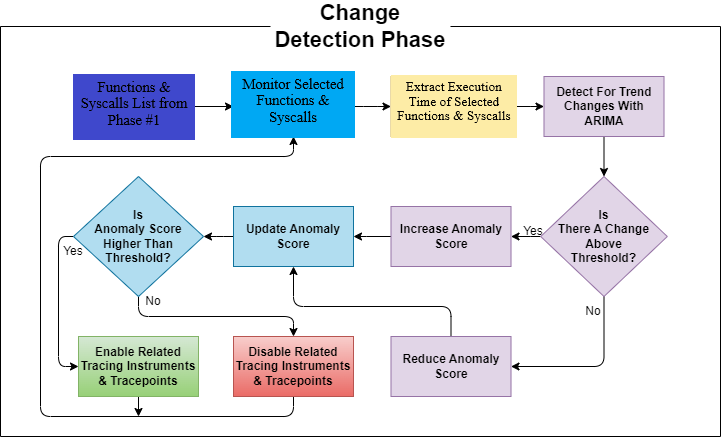
\includegraphics[width=\linewidth]{images/change_detection.png}
  \caption{Change detection phase overview: a pluggable change-detection engine
    (ARIMA(1,1,1) shown) drives the anomaly score, which gates the trace
    configuration.}
  \label{fig:framework_overview}
\end{figure}

\subsection{Phase 1: Tracing-Function Selection}\label{sec:framework:phase1}

\subsubsection{Call-Stack Monitoring}
A suitable snapshot period is determined by the application's characteristics
(e.g., 10 ms for a browser).
The application is executed under representative workloads, and all observed
function and system calls are recorded.

\subsubsection{Family-Group Identification and Sorting}
A \emph{family group} captures the parent--child call hierarchy.
For a snapshot $SP = \{Call\text{-}Stack^i \mid 1 \le i \le n\}$, the
family group of $Call\text{-}Stack^1 = \langle F^a, F^b, F^c \rangle$ is
$\{(F^a, F^b), (F^b, F^c)\}$.
Groups are sorted by invocation frequency, prioritising functions with
the highest potential performance impact.
Algorithm~\ref{alg:familygroup} formalises this procedure.

\begin{algorithm}[tbp]
  \caption{Family-Group Identification \& Sorting}\label{alg:familygroup}
  \begin{algorithmic}[1]
    \State $FG\_List \leftarrow [\,]$; \quad $FG\_Count \leftarrow [\,]$
    \ForAll{$Snapshot \in CallStackSnapshots$}
      \ForAll{$FG \in$ ExtractFamilyGroups($Snapshot$)}
        \If{$FG \notin FG\_List$} append $FG$ to $FG\_List$; set count to 1
        \Else{} increment $FG\_Count[FG]$
        \EndIf
      \EndFor
    \EndFor
    \State Sort $FG\_List$ descending by $FG\_Count$
    \State \Return $FG\_List$
  \end{algorithmic}
\end{algorithm}

\subsubsection{CoV Ranking}
Functions are further ranked by their Coefficient of Variation (CoV) of
execution time $CoV_M = \sigma_M / \mu_M$, ensuring the most volatile
functions are monitored (Algorithm~\ref{alg:covranking}).

\begin{algorithm}[tbp]
  \caption{CoV Ranking of Function Calls}\label{alg:covranking}
  \begin{algorithmic}[1]
    \ForAll{$f \in FunctionExecTimeList$}
      \State $\mu_f \leftarrow$ mean execution time of $f$
      \State $\sigma_f \leftarrow$ standard deviation of $f$
      \State $CoV_f \leftarrow \sigma_f / \mu_f$
    \EndFor
    \State Sort $FunctionExecTimeList$ descending by $CoV$
    \State \Return top-$k\%$ of list (e.g., $k=5$)
  \end{algorithmic}
\end{algorithm}

\subsubsection{List Cutoff}
A cutoff (e.g., top-5\% of all monitored functions) ensures that only the
most performance-critical candidates are tracked, limiting monitoring overhead
without sacrificing coverage of high-impact calls.

\subsection{Phase 2: Change Detection}\label{sec:framework:phase2}

\subsubsection{ARIMA(1,1,1) Model}
For each monitored function, an ARIMA(1,1,1) model predicts the next
execution-time sample based on historical data:
\begin{equation}
  \hat{x}_{t+1} = x_t + \varphi\,\Delta x_t + \theta\,\varepsilon_t,
  \qquad \varepsilon_t = x_t - \hat{x}_t.
  \label{eq:arima}
\end{equation}
First-order differencing captures linear trends; the model flags deviations
from the expected trend without adapting to them, preserving sensitivity to
genuine regime shifts.
A dynamic threshold adaptively scales with recent variability:
\begin{equation}
  \Theta_t = \max\!\bigl(\Theta_{\min},\; k_\sigma \cdot
  \mathrm{std}(\delta_{t-w:t})\bigr),
  \label{eq:dyn_thresh}
\end{equation}
where $\delta_t = |x_t - \hat{x}_t|$, $w = 30$ (lookback window), and
$k_\sigma = 3.0$.
A reading is flagged anomalous when $\delta_t > \Theta_t$.

\textbf{Why ARIMA?}
ARIMA predicts based on past trends and---unlike machine-learning
approaches---does not adapt to new changes, which preserves detection
sensitivity.
ARIMA identifies \emph{all} trend changes regardless of cause
(load shift, anomaly, attack), signalling that additional tracing data
are needed.
We select ARIMA(1,1,1) rather than higher-order variants so that
gradual, organic workload growth is accommodated (the integrated component
re-centres predictions) while quadratic anomalies remain detectable.

\subsubsection{Anomaly Score}
The anomaly score is an exponentially weighted accumulator that rises when
anomalies occur frequently and decays otherwise:
\begin{equation}
  s_t = \beta \cdot \mathbf{1}[\delta_t > \Theta_t]
        + (1 - \beta)\cdot s_{t-1},
  \label{eq:anomscore}
\end{equation}
where $\beta \in (0,1)$ controls the reaction rate.
Tracing is activated when $s_t \geq \theta$ and deactivated when the score
falls below $\theta$.
This gating prevents over-reaction to single spikes while ensuring
persistent anomalies are always captured (see Figure~\ref{fig:response_time}).

\begin{figure}[H]
  \centering
  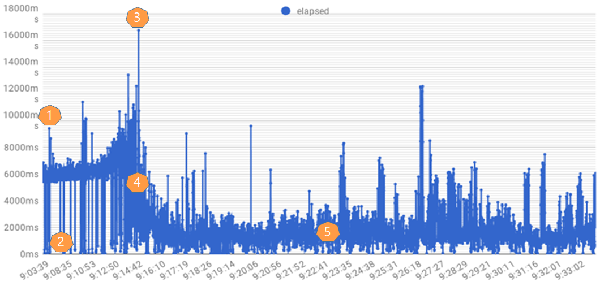
\includegraphics[width=\linewidth]{images/fig_rs.png}
  \caption{Illustrative response-time series with five labelled events.
    A single spike (1) is insufficient to activate tracing; repeated
    anomalies (3) raise the score above threshold; the score must fall
    below threshold (5) before tracing is deactivated.}
  \label{fig:response_time}
\end{figure}

\subsection{Phase 3: Trace Configuration Change}\label{sec:framework:phase3}

When the change-detection phase identifies a trend deviation, tracing is
activated for the associated function family-groups up to a pre-set depth
limit.
At the system level, detected system-call anomalies are mapped to the
corresponding kernel component via the Linux system-call table~\cite{valsorda-no-date},
enabling targeted kernel-level tracing.
Algorithm~\ref{alg:changedetect} combines all three decisions into a single
online loop.

\begin{algorithm}[tbp]
  \caption{Online Change Detection and Trace Gating}\label{alg:changedetect}
  \begin{algorithmic}[1]
    \State Initialise $s_t \leftarrow 0$ for all monitored functions
    \ForAll{incoming sample $x_t$ per function}
      \State $\hat{x}_t \leftarrow \text{ARIMA}(x_{t-1}, x_{t-2}, \ldots)$
      \State $\delta_t \leftarrow |x_t - \hat{x}_t|$
      \State $\Theta_t \leftarrow \max(\Theta_{\min},\; k_\sigma \cdot \mathrm{std}(\delta_{t-w:t}))$
      \State $s_t \leftarrow \beta \cdot \mathbf{1}[\delta_t > \Theta_t] + (1-\beta)\cdot s_{t-1}$
      \If{$s_t \geq \theta$}
        \State Enable tracepoint(s) for this function's family-group
      \Else
        \State Disable tracepoint(s)
      \EndIf
    \EndFor
  \end{algorithmic}
\end{algorithm}

% ===================================================================
\section{Prior Qualitative Evaluation}\label{sec:casestudies}
% ===================================================================

The conference paper~\cite{10197790} validated the framework through four
case studies on Firefox and a controlled Apache server.
These were \emph{illustrative demonstrations}: in each case, a known Bugzilla
performance-bug report was used post~hoc to confirm that the framework ranked
the responsible function highly and triggered tracing at the correct time
windows.
Table~\ref{tab:casestudy_summary} summarises the key results; the subsections
below restore the concrete metric-level findings that are most informative
for practical deployment.

\begin{table}[tbp]
\centering
\resizebox{\columnwidth}{!}{%
\begin{tabular}{llccc}
\toprule
\textbf{Case} & \textbf{Bug / Scenario} & \textbf{Detected?} &
  \textbf{Candidate-list overhead} & \textbf{ARIMA storage reduction} \\
\midrule
1 & Apache CPU/disk/network trend changes & Yes (21/35 metrics) & 66\% (nmon metric selection) & --- \\
2 & Firefox VSync driver slowdown (PDF load) & Yes (rank 14 of 8,231) & 95\% (CoV cutoff, 410 monitored) & 44\% \\
3 & Firefox 3D-rendering slowdown & Yes (rank 6) & 95\% (CoV cutoff) & --- \\
4 & Firefox startup slowdown (DNS failure) & Yes (\texttt{\_\_\_sys\_sendmsg} $\to$ \texttt{net/socket.c}) & 95\% (CoV cutoff) & Multi-level detection \\
\bottomrule
\end{tabular}%
}
\caption{Summary of four qualitative case studies from~\protect\cite{10197790}.
  All overhead reductions are relative to always-on monitoring of the
  full candidate set.}
\label{tab:casestudy_summary}
\end{table}

These case studies confirm that the framework correctly narrows a large
candidate space to a tractable monitored set, that the anomaly-score
mechanism triggers and releases tracing at appropriate times, and that
multi-level (application + kernel) detection is feasible.
Rigorous prospective evaluation at scale is what motivates the remainder
of this paper.

% -------------------------------------------------------------------
\subsection{Case Study 1: System-Level Overhead Characterisation}\label{sec:cs1}
% -------------------------------------------------------------------

The first case study monitored a PHP/Apache server under escalating concurrent
load using nmon at a 1-second sampling rate (\texttt{nmon -f -s 1 -c 3600},
run for one hour).
A total of \textbf{35 system-level metrics} spanning CPU, memory, disk, and
network categories were recorded.
ARIMA change detection flagged \textbf{21 of the 35 metrics} as exhibiting
trend deviations---not simultaneously, but at distinct time windows
corresponding to each load increment.

\textbf{Runtime overhead.}
nmon's CPU utilisation overhead was measured in two configurations: (i) with
all 35 metrics active against a baseline CPU utilisation of up to 9\%, and
(ii) after the preliminary monitoring stage discarded metrics whose CoV
ranking placed them outside the selective set.
In configuration (i), nmon added an average of \textbf{0.3\%} additional CPU
utilisation (maximum 0.7\%; minimum near 0\%), yielding a total
system overhead of 6.8\% relative to the no-nmon baseline.
Because nmon's CPU cost is static per sampling rate, this overhead would
reduce proportionally as baseline CPU utilisation rises.
In configuration (ii), selective metric monitoring reduced nmon's own
average CPU contribution by 0.2\%---a \textbf{66\% reduction} in the monitoring
tool's CPU overhead relative to the 0.3\% all-metrics baseline, alongside a
4.3\% reduction in total system CPU overhead.

These numbers establish the practical deployment cost of the framework's
system-level monitoring tier: sub-percent CPU overhead in a low-utilisation
server environment, with two-thirds of that cost eliminated by applying the
CoV-based metric selection.

% -------------------------------------------------------------------
\subsection{Case Study 2: Candidate-Space Narrowing and Trace Gating}\label{sec:cs2}
% -------------------------------------------------------------------

The second case study reproduced a Bugzilla-reported Firefox performance
regression~\cite{clessili-2022}: loading a large PDF caused the browser to
stall at the VSync driver synchronisation call.
The pre-testing profiling phase (20-minute load/stress cycle with 50\,MB and
500\,KB PDF files; call stacks recorded by \texttt{perf}) discovered
\textbf{8,231 unique function/system-call family-groups}.
Applying the 5\% CoV-ranking cutoff reduced this to a \textbf{monitored list
of 410 candidates}---a 95\% reduction in the set that receives active tracing.

The known culprit, \texttt{mozilla::VsyncRefreshDriverTimer::RunRefreshDrivers},
held \textbf{rank 14} on this 410-item list.
Its execution time remained well below 20\,ms when loading the smaller
(500\,KB) PDF; under the larger PDF, the function exhibited \textbf{bursts
exceeding 500\,ms}, which ARIMA flagged as anomalous.
The anomaly-score gating reduced the fraction of test time for which
the culprit tracepoint was actively recording by \textbf{44\%} compared to
always-on tracing, directly reducing stored trace volume.

Figure~\ref{fig:cs2_tracegate} illustrates the execution-time trace and the
corresponding adaptive decision for the culprit tracepoint.
The left panel shows the ARIMA prediction alongside measured execution times;
the right panel shows time windows where the anomaly score crossed threshold
and tracing was activated.

\begin{figure*}[tbp]
     \centering
     \begin{subfigure}[ht]{0.49\textwidth}
         \centering
         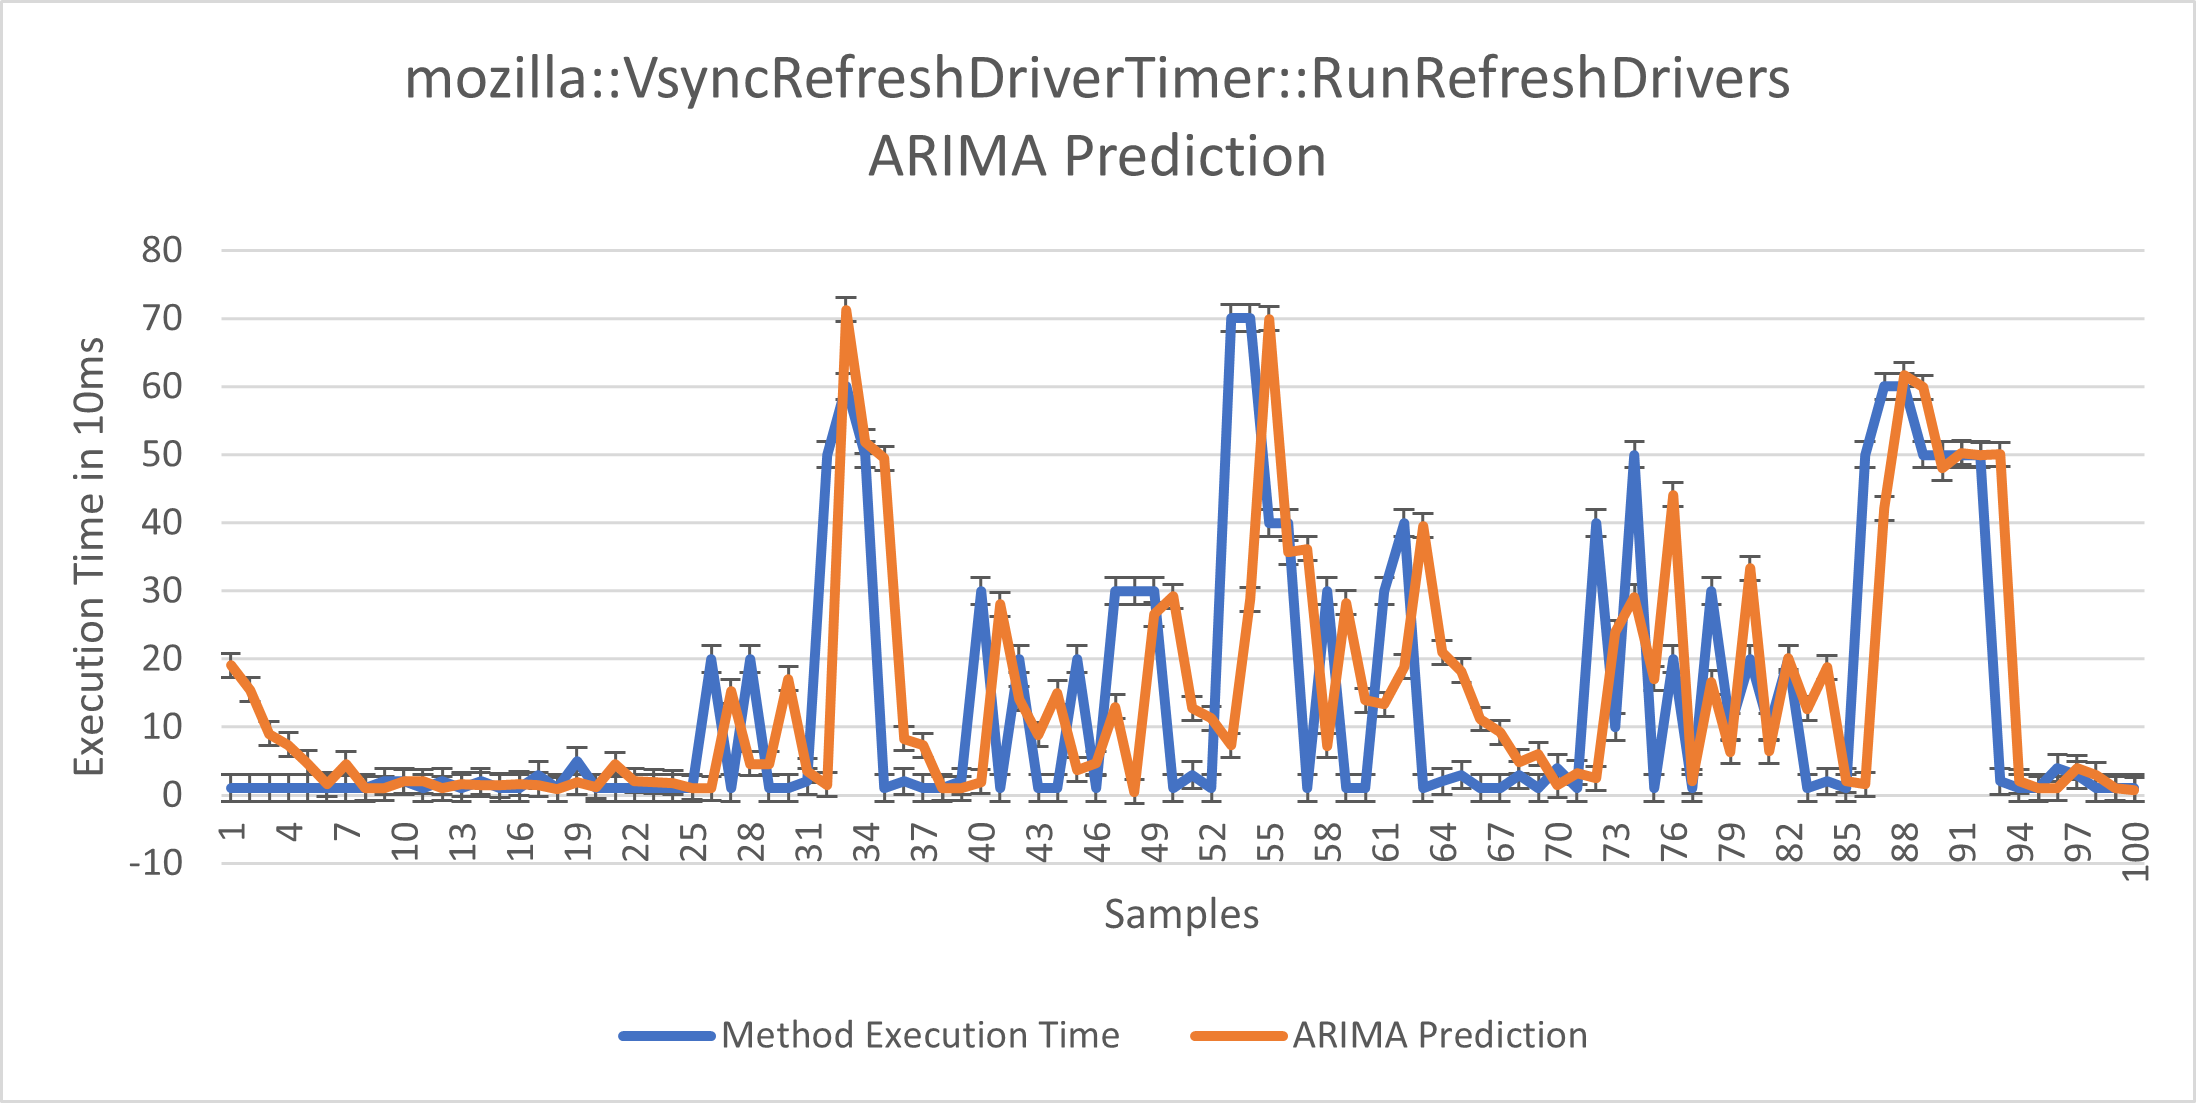
\includegraphics[width=\textwidth]{images/cs2_l1.png}
         \caption{Execution Time \& ARIMA Prediction for
           \texttt{mozilla::VsyncRefreshDriverTimer::RunRefreshDrivers}.}
         \label{fig:cs2_l1}
     \end{subfigure}
     \hfill
     \begin{subfigure}[ht]{0.49\textwidth}
         \centering
         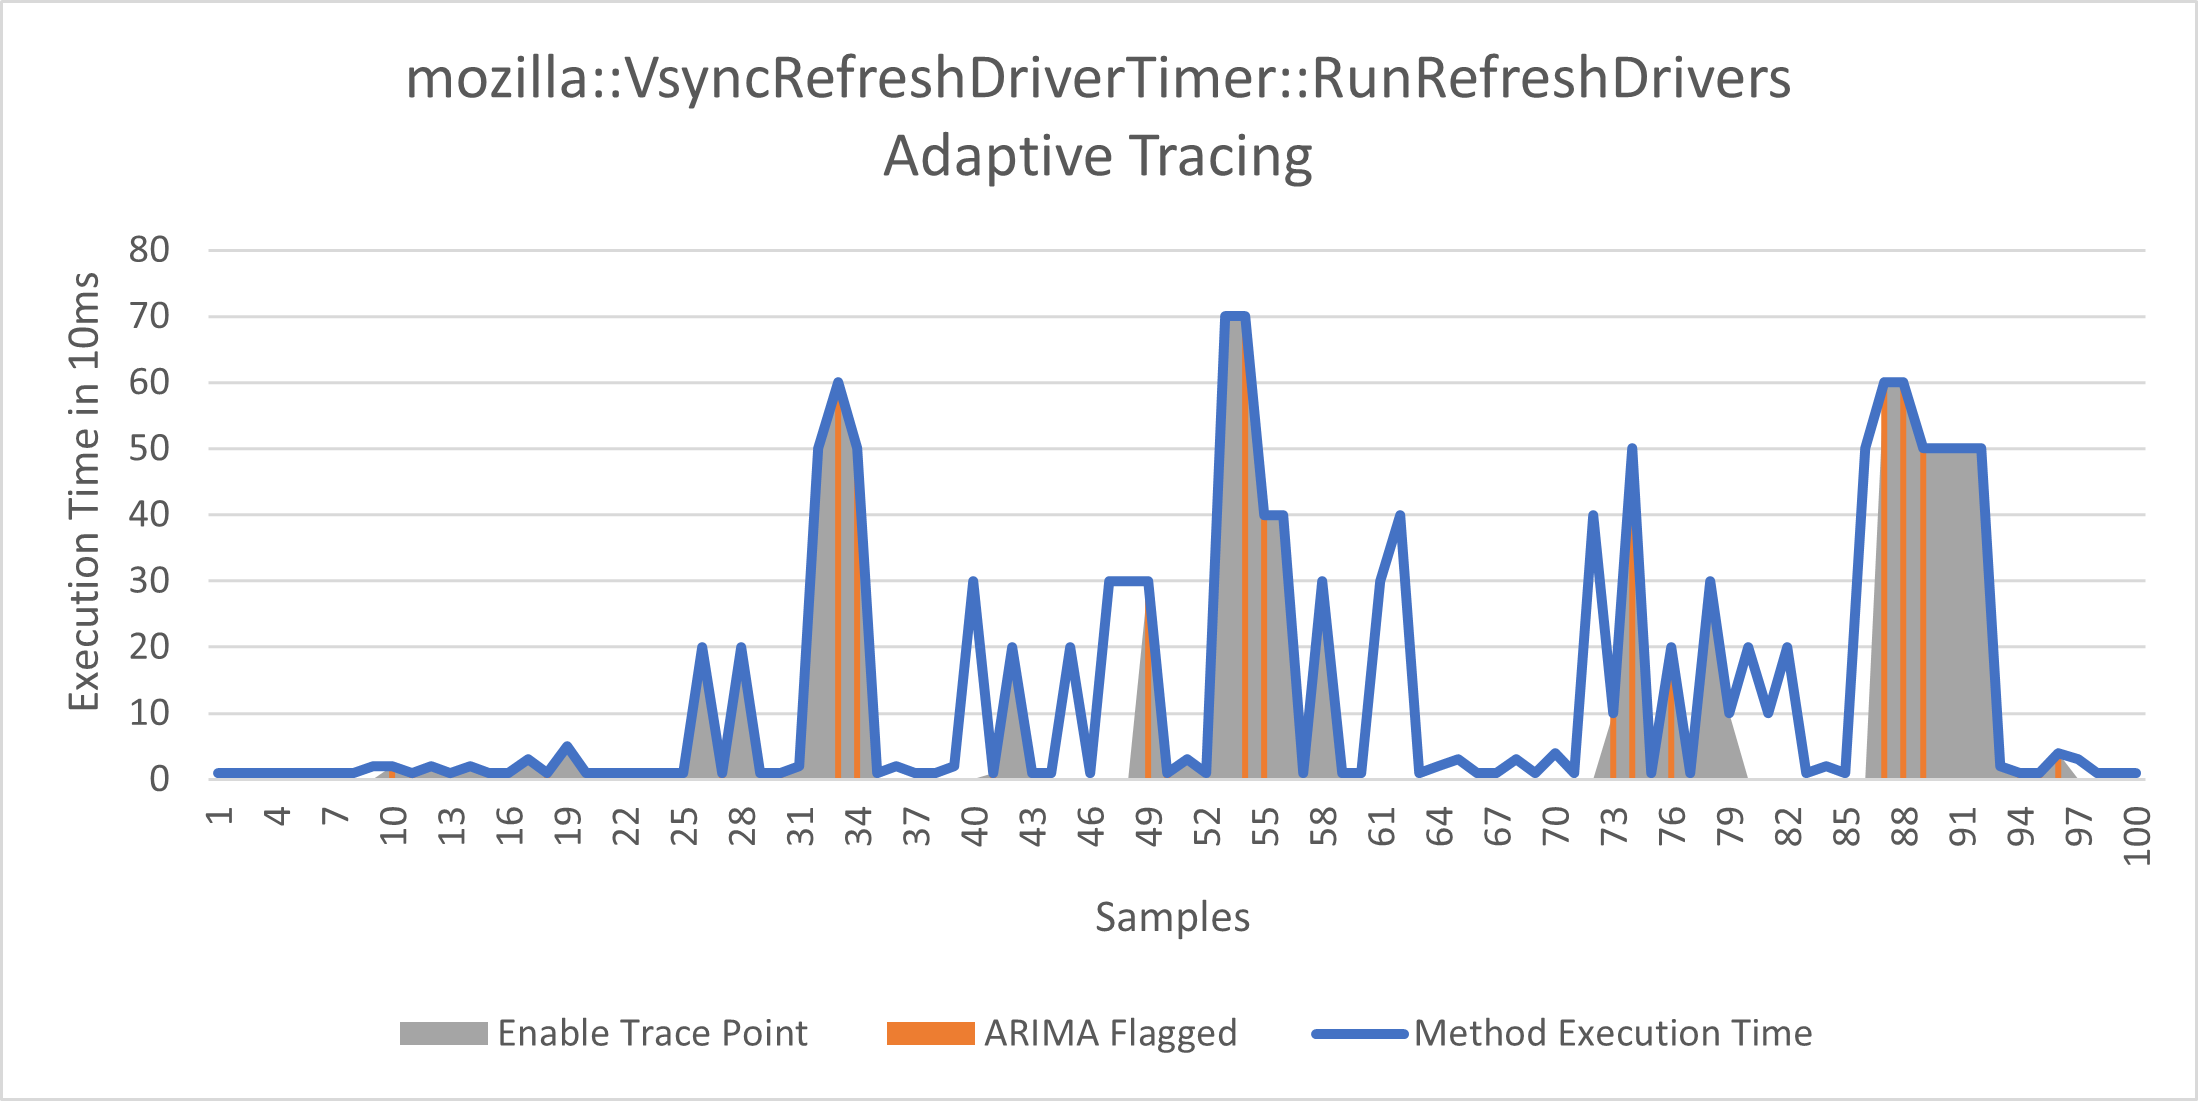
\includegraphics[width=\textwidth]{images/cs2_l2.png}
         \caption{Adaptive tracepoint gate: ON intervals correspond to anomaly-score
           exceedances; 44\% of test time is suppressed.}
         \label{fig:cs2_l2}
     \end{subfigure}
     \caption{Case Study 2 --- trace-gating behaviour on the known VSync culprit
       (Firefox large-PDF scenario~\cite{clessili-2022}).
       Shaded regions in the right panel indicate active tracing intervals.
       Execution-time bursts exceeding 500\,ms trigger the gating mechanism.}
     \label{fig:cs2_tracegate}
\end{figure*}

% -------------------------------------------------------------------
\subsection{Case Study 3: Class-Level Fault Localisation}\label{sec:cs3}
% -------------------------------------------------------------------

The third case study targeted a Bugzilla report of extremely slow 3D CSS
transformation rendering in Firefox~\cite{muizelaar-2020}, attributed to the
class \texttt{WebRenderCommandBuilder}.
The profiling phase (15-minute 3D-animation stress cycle) yielded 15,934 unique
function family-groups; the 5\% cutoff produced a 797-item monitored list.

The culprit function, \texttt{CreateWebRenderCommandsFromDisplayList},
ranked \textbf{6th} on the monitored list.
The framework derived the owning class from the call stack and identified
\textbf{\texttt{mozilla::layers::WebRenderCommandBuilder}} as the responsible
class---an \textbf{exact match} to the Bugzilla report's named class.
This result demonstrates that the CoV ranking is sufficient to surface
class-level fault attribution without enumerating all 15,934 family-groups:
the culprit appeared in the top 0.04\% of the full candidate space.

% -------------------------------------------------------------------
\subsection{Case Study 4: Kernel-Level System-Call Mapping}\label{sec:cs4}
% -------------------------------------------------------------------

The fourth case study reproduced a Firefox startup slowdown caused by
DNS-resolution failure~\cite{cook-2022}.
The profiling phase (15-minute load cycle with alternating DNS configurations)
produced 5,764 unique family-groups; the 5\% cutoff yielded 289 monitored items.

The framework flagged the system call \textbf{\texttt{\_\_\_sys\_sendmsg}}
(rank 236 on the monitored list) as anomalous during the DNS-failure scenario.
This system call was then mapped via a Linux system call
table~\cite{valsorda-no-date} to the kernel component
\textbf{\texttt{net/socket.c}}---the Linux network socket subsystem.
Cross-referencing against the Bugzilla report confirmed an \textbf{exact
alignment}: the DNS-resolution failure manifests through network socket
operations, precisely the subsystem identified by the framework.

This case study provides unusually direct evidence that the DAET framework
supports true multi-level tracing: a high-level symptom (slow Firefox startup)
is traced through the application call stack to a specific system call and from
there to the kernel subsystem responsible for the observed behaviour, all
without requiring the developer to scan the full 5,764-item candidate space
manually.

% ===================================================================
\section{Large-Scale Comparative Evaluation}\label{sec:largescale}
% ===================================================================

\subsection{Dataset}\label{sec:largescale:dataset}

We use two publicly available Mozilla Treeherder performance-telemetry
datasets~\cite{mozillatreeherder}.
Treeherder is Mozilla's continuous-integration platform; it records
performance signatures for each test suite across every Firefox build
and raises \emph{regression alerts} when a Bayesian change-point detector
flags a statistically significant performance change.

The raw Firefox-Android dataset contains 17,989 total alert records across
342 unique telemetry signatures.

\textbf{Canonical evaluation pipeline} (Section~\ref{sec:three_way},
implemented in \texttt{run\_full\_evaluation.py}).
Signatures from both repositories are retained if the time-series contains
at least 30 data points, and they are split chronologically 60\%/20\%/20\%
(train / held-out validation / test) with no information from the validation
or test portions used during training.
This yields \textbf{342} Firefox-Android and \textbf{1{,}477} mozilla-beta
matched signatures; the 20\% test window contains 136 and 395 alerted
signatures, respectively.

\textbf{Calibration baseline} (Section~\ref{sec:largescale:RQ1},
for prior-work comparison with~\cite{10197790}).
Firefox-Android signatures are retained under a stricter 50-point length
filter and split 70\%/30\% (train/test).
SMA~$w$ and EWMA~$\alpha$ were set from exploratory analysis of this
dataset without an independent held-out validation set---an acknowledged
limitation detailed in Section~\ref{sec:threats}.
After filtering, \textbf{214 matched signatures} remain with
\textbf{7,612 regression-alert records} and 150 alerted signatures in the
test set.
Table~\ref{tab:dataset} summarises both configurations.

\begin{table}[tbp]
\centering
\resizebox{\columnwidth}{!}{%
\begin{tabular}{lrr}
\toprule
\textbf{Property} & \textbf{Firefox-Android} & \textbf{mozilla-beta} \\
\midrule
Total alert records (raw)     & 17{,}989  & 3{,}597     \\
Matched signatures (used)     & 342       & 1{,}477 \\
Mean time-series length       & 625.9     & 801.4   \\
Signatures w/ test-set alerts & 136       & 395     \\
\bottomrule
\end{tabular}%
}
\caption{Mozilla Treeherder dataset configurations.
  \emph{Canonical pipeline} (Section~\ref{sec:three_way}): 60\%/20\%/20\%
  chronological split, 30-point length filter, independent held-out
  validation for HP tuning.
  \emph{Calibration baseline} (Section~\ref{sec:largescale:RQ1}):
  70\%/30\% split on Firefox-Android only, 50-point filter, no independent
  validation hold-out --- retained for prior-work comparison.}
\label{tab:dataset}
\end{table}

\subsection{Competing Change Detectors}\label{sec:largescale:detectors}

We compare five change-detection engines, all embedded in the same DAET
framework with identical anomaly-score gating (Eq.~\ref{eq:anomscore}):

\textbf{ARIMA(1,1,1)} (parametric benchmark engine from~\cite{10197790}): uses Eq.~\ref{eq:arima} for
prediction, with a dynamic threshold (Eq.~\ref{eq:dyn_thresh}).
Requires training on the first 70\% of each series; rolling ARIMA window
of 60 samples with minimum history 20 samples.
Models are fitted using the \texttt{statsmodels} library
(v0.13+,~\cite{seabold2010statsmodels}) in Python with fixed order
$(p,d,q)=(1,1,1)$ across all signatures.
When fewer than 20 historical samples are available, the detector falls
back to LAST until the minimum window is reached.

\textbf{LAST}: the trivially simple ``predict the last observed value''
baseline, $\hat{x}_{t+1} = x_t$.
No training required.

\textbf{SMA(w=20)}: simple moving average over the last $w=20$ samples.
Smoothes random noise by averaging recent values.

\textbf{EWMA($\alpha=0.30$)}: exponentially weighted moving average,
$\hat{x}_{t+1} = \alpha x_t + (1-\alpha)\hat{x}_t$.
Places exponentially decreasing weight on older observations.
The smoothing parameter $\alpha=0.30$ was set by the same exploratory
analysis that guided the ARIMA defaults; it was not independently tuned
on a held-out validation set, which is acknowledged as a limitation
in Section~\ref{sec:threats}.

All four statistical methods share the same anomaly-score parameters
($\beta = 0.30$, $\theta = 0.30$) and tolerance window ($\tau = 5$ samples).
For each method, the binary ``anomaly'' signal is determined by
$|\delta_t| > \Theta_t$, where $\Theta_t$ uses the rolling-window dynamic
threshold (Eq.~\ref{eq:dyn_thresh}).

\subsection{Calibration-Baseline Protocol}\label{sec:largescale:protocol}

The following protocol applies to the calibration baseline only (214
signatures, 70\%/30\% split).  The canonical protocol is described in
Section~\ref{sec:three_way}.

For each of the 214 signatures and each of the 4 statistical detectors, we:
(1)~fit the model on the first 70\% of the time series;
(2)~run the detector on the remaining 30\% (test set) in a single pass;
(3)~align the binary detect/no-detect output with ground-truth alert
timestamps using a tolerance window of $\tau = 5$ samples either side
(an alert within $\pm5$ samples of a detection is counted as a true positive);
(4)~compute precision, recall, F1, false-alarm rate (FAR), and storage reduction.
All metrics are \emph{macro-averaged}: computed per signature and then
aggregated to a mean across the 214 signatures.

The \emph{detection delay} for a matched alert at time $t_a$ is defined as
$d = s - t_a$, where $s$ is the start time-step of the earliest detected
interval that covers $[t_a - \tau,\; t_a + \tau]$; a negative delay indicates
pre-detection (the detector fires before the centre of the alert window).
The \emph{false-alarm rate} (FAR) is an interval-level rate:
\begin{equation*}
  \text{FAR} = \frac{\text{fp\_iv}}{T_{\text{test}}},
\end{equation*}
where $\text{fp\_iv}$ is the number of false-alarm activation intervals
(maximal contiguous trace-ON periods whose $\pm\tau$ neighbourhood contains
no ground-truth alert), and $T_{\text{test}}$ is the total number of test-set
samples.  Because mean interval durations on this dataset are approximately
one sample, FAR values are numerically close to a sample-level rate
$\text{FP}_{\text{samples}}/T_{\text{test}}$, but the denominator is sample
count while the numerator counts intervals, not individual samples.
When multiple detector activations fall within $\tau$ samples of the same
alert, only one true-positive interval is counted; additional activations within
that window form separate false-alarm intervals.
The \emph{detection rate} is the fraction of the 150 signatures that have
$\geq 1$ alert in the test set and for which at least one alert is detected.

\subsection{RQ1: Calibration-Baseline Results (70\%/30\%)}\label{sec:largescale:RQ1}

\noindent\fbox{\parbox{\columnwidth}{\small\textbf{Calibration baseline only.}
These results use the 70\%/30\% split with 214 Firefox-Android signatures
and no held-out validation set for SMA/EWMA tuning.
The canonical primary results are in
Section~\ref{sec:three_way} (Tables~\ref{tab:three_way_fa}--\ref{tab:three_way_mb}).
}}

\medskip
Table~\ref{tab:main_results} reports the aggregate evaluation metrics.
Standard deviations across 214 signatures are given in parentheses.

\begin{table}[tbp]
\centering
\resizebox{\columnwidth}{!}{%
\begin{tabular}{lcccccc}
\toprule
\textbf{Method} & \textbf{Precision} & \textbf{Recall} & \textbf{F1} &
  \textbf{FAR} & \textbf{Det.\ Rate (\%)} & \textbf{Storage Red.\ (\%)} \\
\midrule
ARIMA(1,1,1) & 0.106 (0.17) & 0.606 (0.45) & 0.174 (0.23) &
  0.053 (0.01) & 88.67 & 89.75 \\
LAST         & 0.079 (0.15) & 0.484 (0.45) & 0.133 (0.19) &
  \textbf{0.052 (0.01)} & 72.67 & 89.42 \\
SMA(w=20)    & \textbf{0.112 (0.17)} & \textbf{0.657 (0.44)} &
  \textbf{0.186 (0.23)} & \textbf{0.052 (0.01)} & \textbf{96.00} & 88.83 \\
EWMA($\alpha$=0.30) & 0.090 (0.16) & 0.562 (0.45) & 0.151 (0.21) &
  0.056 (0.01) & 82.67 & \textbf{91.00} \\
\bottomrule
\end{tabular}%
}
\caption{\textbf{Calibration-baseline} results (214 Firefox-Android signatures,
  70\%/30\% split, SMA/EWMA parameters from exploratory analysis).
  Canonical primary results are in Tables~\ref{tab:three_way_fa}--\ref{tab:three_way_mb}.
  Bold marks the best value per column.
  $n_{\text{alert}}=150$ signatures have $\geq 1$ alert in the test set.
  \emph{Note:} the ablation section (Section~\ref{sec:ablation}) uses a
  stricter regression-only ground truth; ablation values at the same
  defaults are numerically lower and are not directly comparable to this table.}
\label{tab:main_results}
\end{table}

Table~\ref{tab:compute_cost} reports the total runtime and peak memory
footprint for all five detectors over the 214-signature evaluation.

\begin{table}[tbp]
\centering
\resizebox{\columnwidth}{!}{%
\begin{tabular}{lccc}
\toprule
\textbf{Method} & \textbf{Total Runtime (s)} & \textbf{Mean Peak Mem.\ (KB/sig)} & \textbf{Relative Runtime} \\
\midrule
ARIMA(1,1,1)        & 807   & 1,423 & 27$\times$ \\
SMA(w=20)           & 30    & 90    & 1$\times$ (baseline) \\
EWMA($\alpha$=0.30) & 24    & 84    & 0.8$\times$ \\
LAST                & 24    & 84    & 0.8$\times$ \\
\bottomrule
\end{tabular}%
}
\caption{Computational cost over 214 Mozilla Firefox-Android signatures
  for the four statistical detectors.
  All experiments were conducted on a CPU-only Windows workstation
  (Intel Core i7, 16\,GB RAM) running Python~3.12 with PyTorch~2.4.1+cpu;
  no GPU acceleration was used.
  Runtime is wall-clock time for the full 214-signature evaluation pass.
  Peak memory is the mean per-signature OS-reported peak RSS.
  ARIMA incurs a 27$\times$ runtime overhead and 16$\times$ memory overhead
  relative to SMA, with no statistically significant accuracy gain
  (Table~\ref{tab:wilcoxon}).}
\label{tab:compute_cost}
\end{table}

\textbf{Key observations.}
(i)~SMA achieves the highest recall (0.657), F1 (0.186), and detection rate (96.0\%),
making it the strongest statistical detector on this benchmark.
(ii)~EWMA achieves the highest storage reduction (91.0\%) through a more conservative
activation policy, but at the cost of lower detection rate (82.67\%) and recall (0.562).
(iii)~ARIMA achieves detection rate 88.67\% and F1 0.174, significantly ahead of
LAST and EWMA; however, it costs 27$\times$ more runtime and 16$\times$ more
memory than SMA (Table~\ref{tab:compute_cost}) with no statistically significant
accuracy gain over SMA in F1 or precision.
(iv)~Precision is low ($<0.12$) across all four methods.
\textbf{What ``false positive'' means here.}
Under the Treeherder-agreement benchmark, a DAET detection is counted as
a \emph{false positive} if its alert window was not matched by any
Treeherder alert under the paper's temporal alignment rule.
This does \emph{not} mean the detection was factually wrong---only that
Mozilla's Bayesian alerting system did not produce a coincident alert.
Treeherder may miss transient regressions or include alerts from
infrastructure changes; many DAET detections counted as false positives
may therefore correspond to genuine but unlabelled performance excursions.
All reported precision values measure \emph{Treeherder-agreement}, not
ground-truth anomaly validity.
No manual adjudication or second validation source is available to
distinguish these cases; true anomaly precision is therefore unknown.
(v)~Detection delay: SMA fires pre-emptively with mean delay $-3.2$ samples;
ARIMA shows delay $-2.8$ samples.

Figure~\ref{fig:comparison_bars} summarises the aggregate metrics visually.
Figure~\ref{fig:result_sample} shows representative detection outputs for one
Mozilla signature under all four statistical detectors.

\begin{figure}[H]
  \centering
  \begin{subfigure}[t]{\linewidth}
    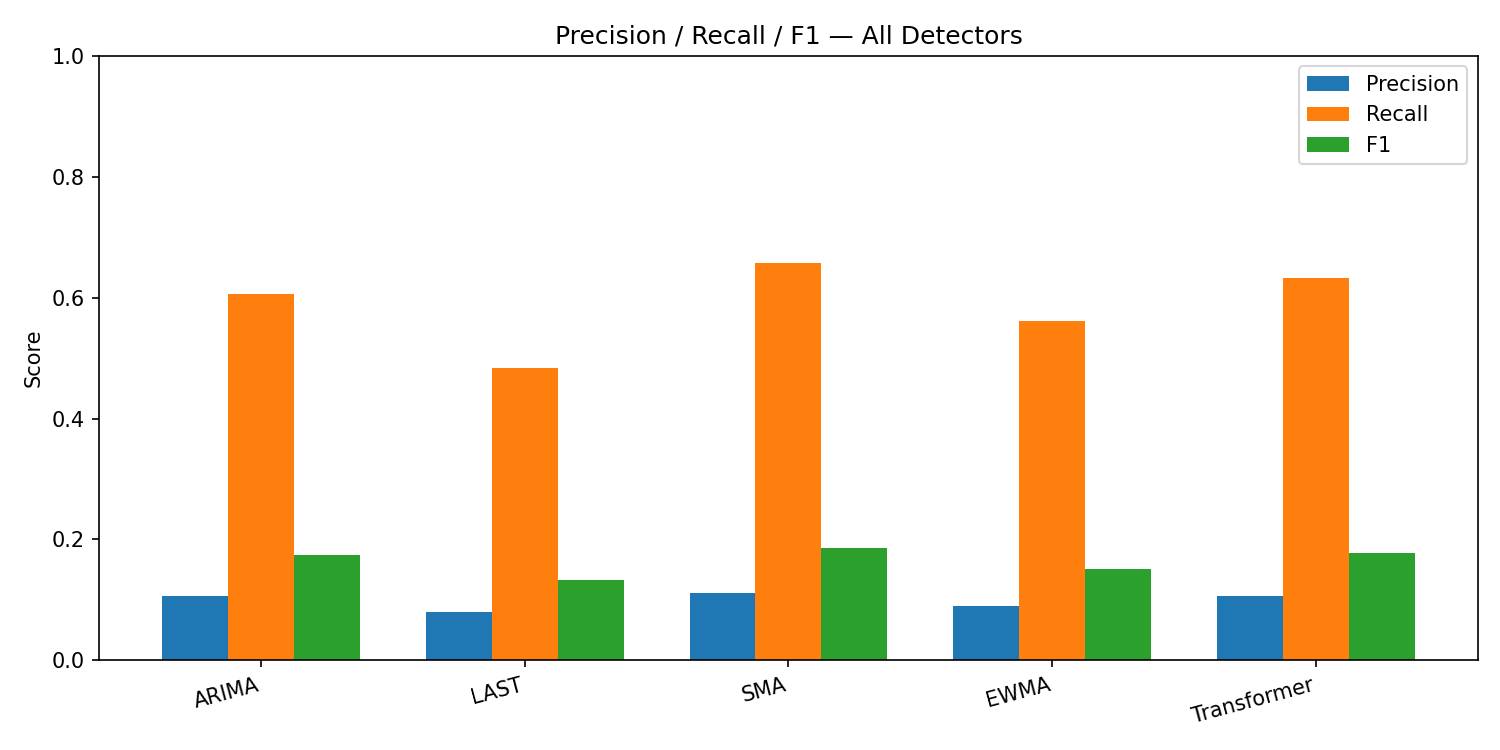
\includegraphics[width=\linewidth]{images/comparison_precision_recall_f1.png}
  \caption{Precision, Recall, and F1 across the four statistical detectors.}
    \label{fig:cmp_prf}
  \end{subfigure}
  \\[4pt]
  \begin{subfigure}[t]{0.49\linewidth}
    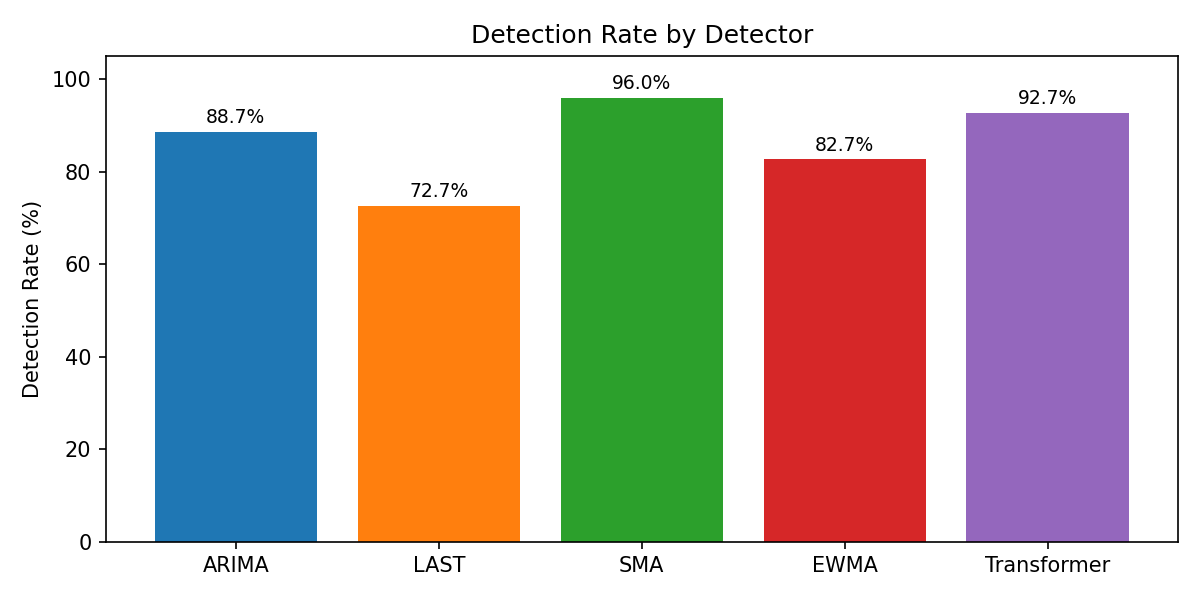
\includegraphics[width=\linewidth]{images/comparison_detection_rate.png}
    \caption{Detection Rate (\%).}
    \label{fig:cmp_det}
  \end{subfigure}
  \hfill
  \begin{subfigure}[t]{0.49\linewidth}
    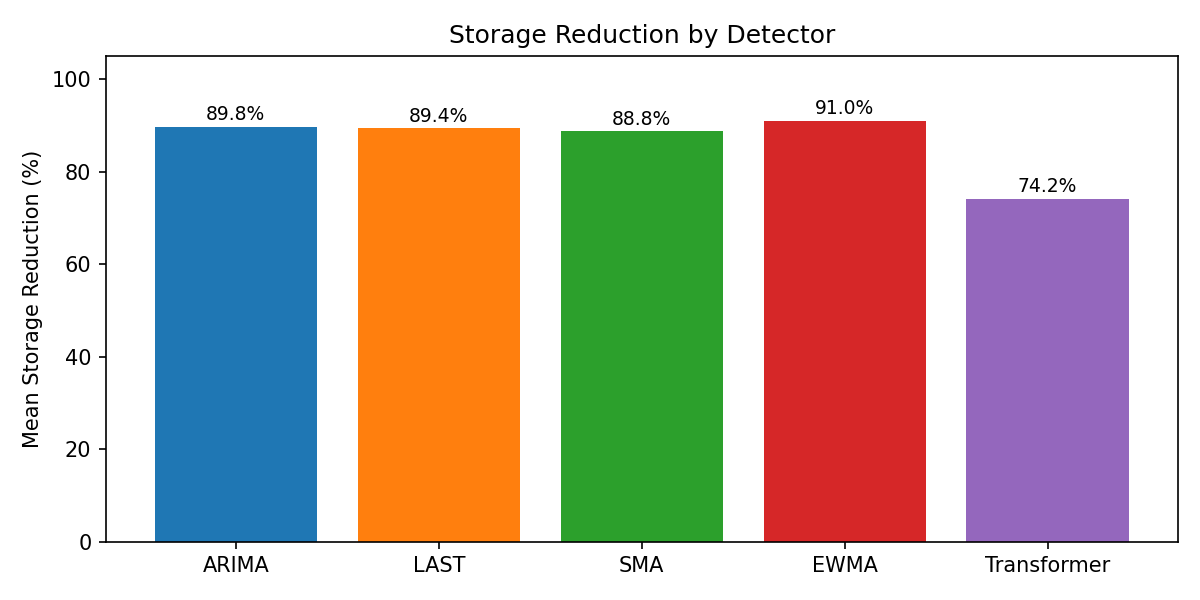
\includegraphics[width=\linewidth]{images/comparison_storage_reduction.png}
    \caption{Storage Reduction (\%).}
    \label{fig:cmp_stor}
  \end{subfigure}
  \caption{Aggregate metric comparison across the four statistical detectors
    (214 Firefox-Android signatures, 70\%/30\% split).
    SMA leads on precision, F1, recall, and detection rate;
    EWMA achieves the highest storage reduction.}
  \label{fig:comparison_bars}
\end{figure}

\begin{figure*}[tbp]
  \centering
  \begin{subfigure}[t]{0.49\textwidth}
    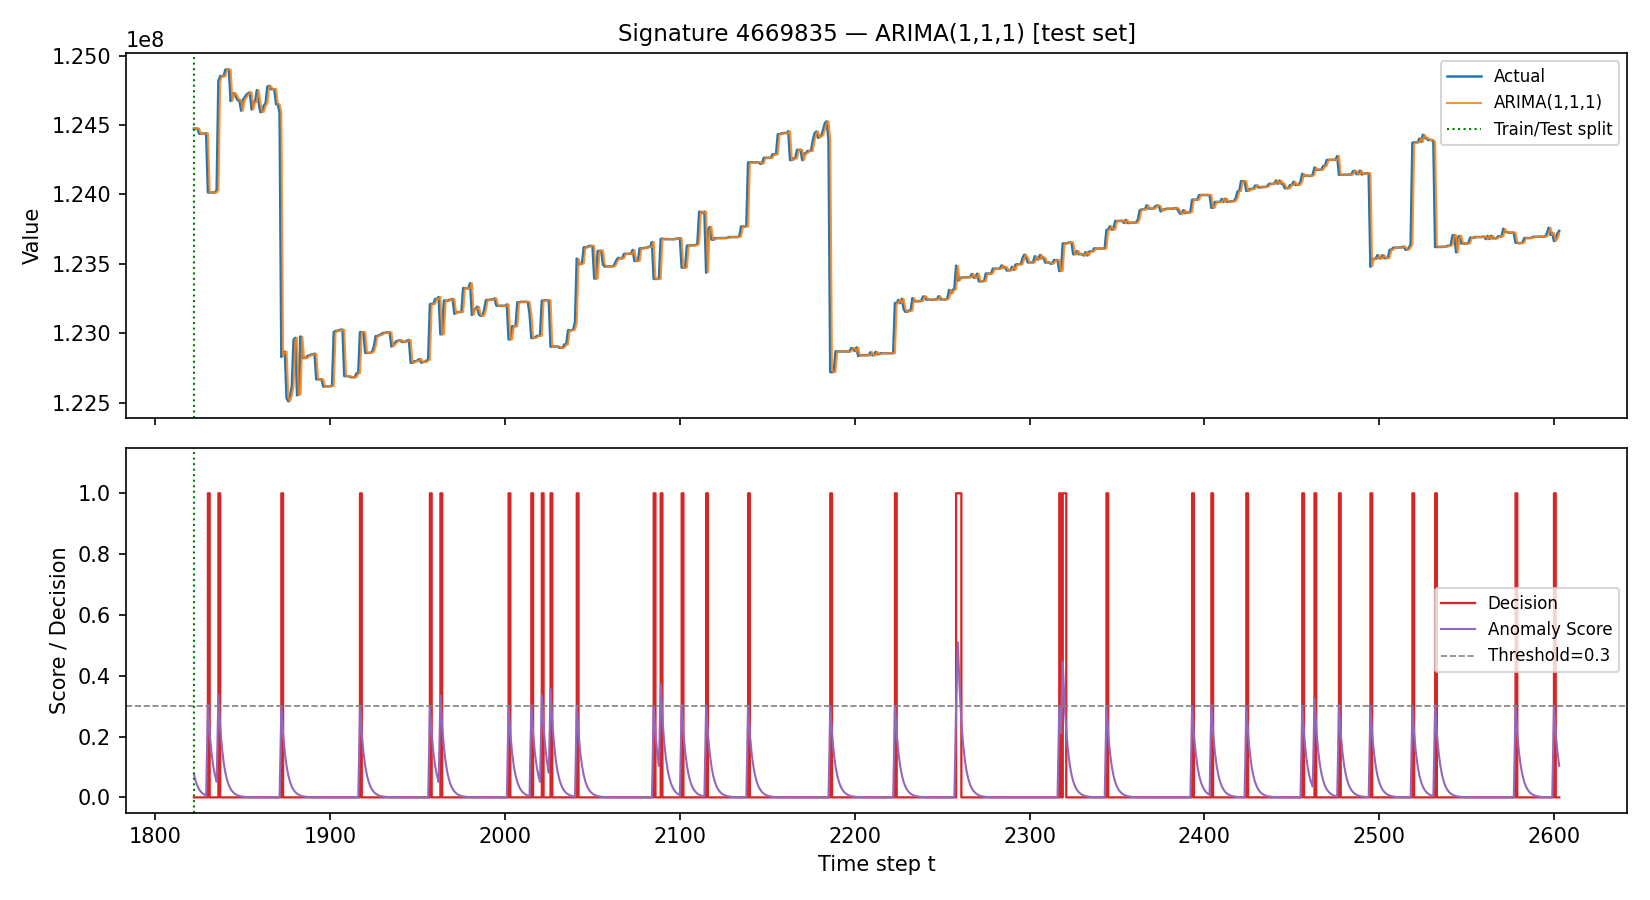
\includegraphics[width=\textwidth]{images/results_plots/4669835_arima.png}
    \caption{ARIMA(1,1,1)}
    \label{fig:sample_arima}
  \end{subfigure}
  \hfill
  \begin{subfigure}[t]{0.49\textwidth}
    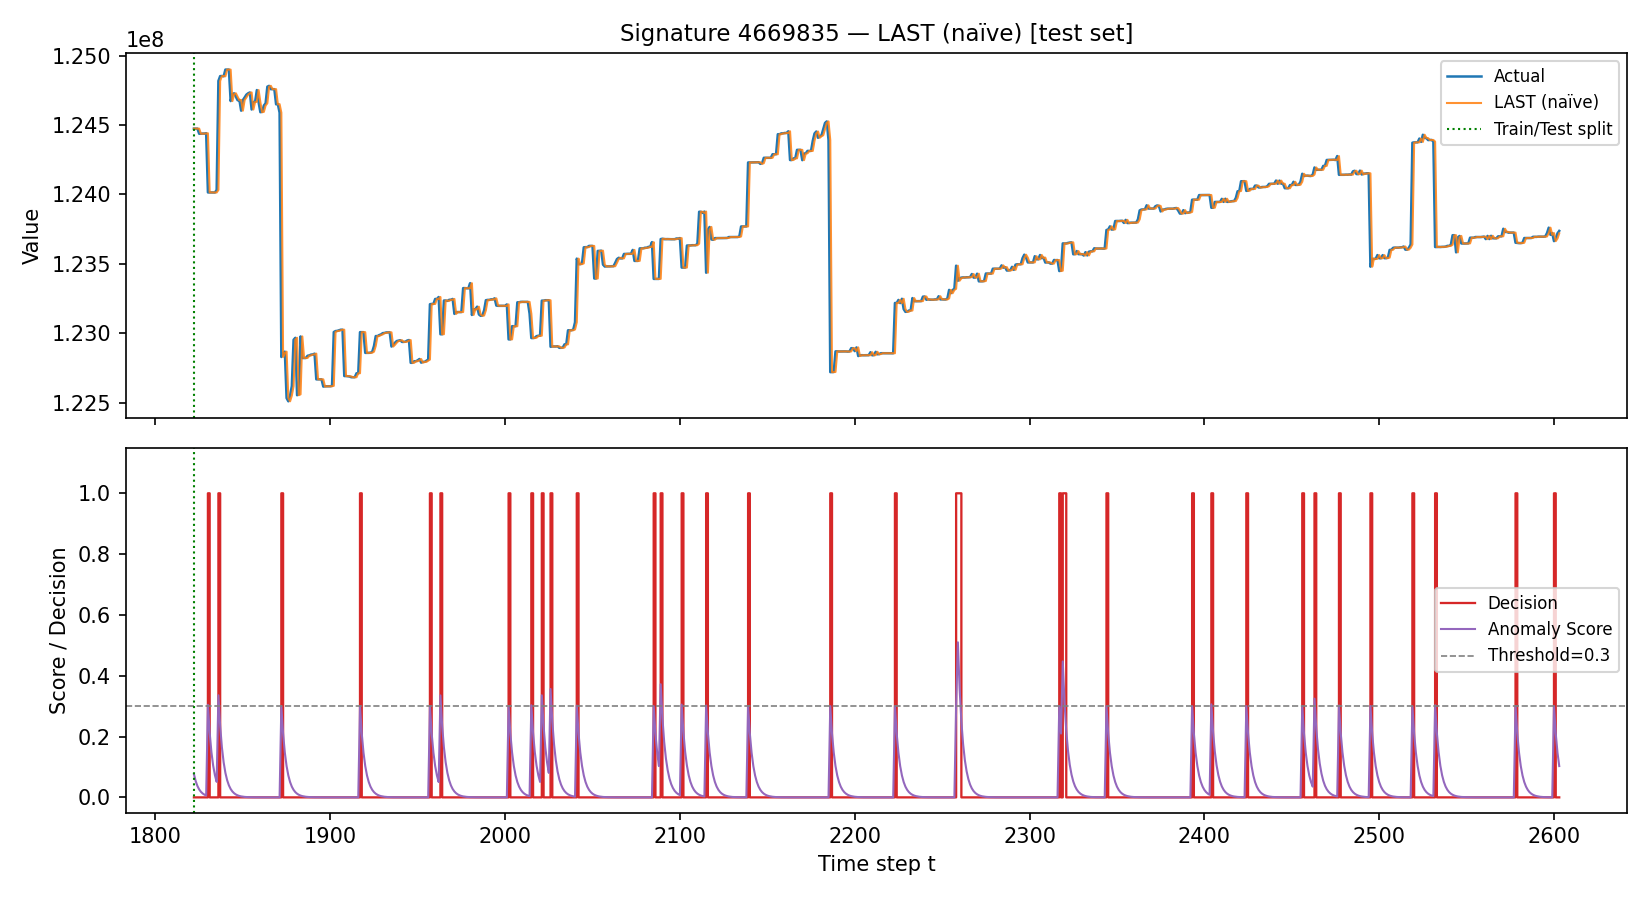
\includegraphics[width=\textwidth]{images/results_plots/4669835_last.png}
    \caption{LAST}
    \label{fig:sample_last}
  \end{subfigure}
  \\[6pt]
  \begin{subfigure}[t]{0.49\textwidth}
    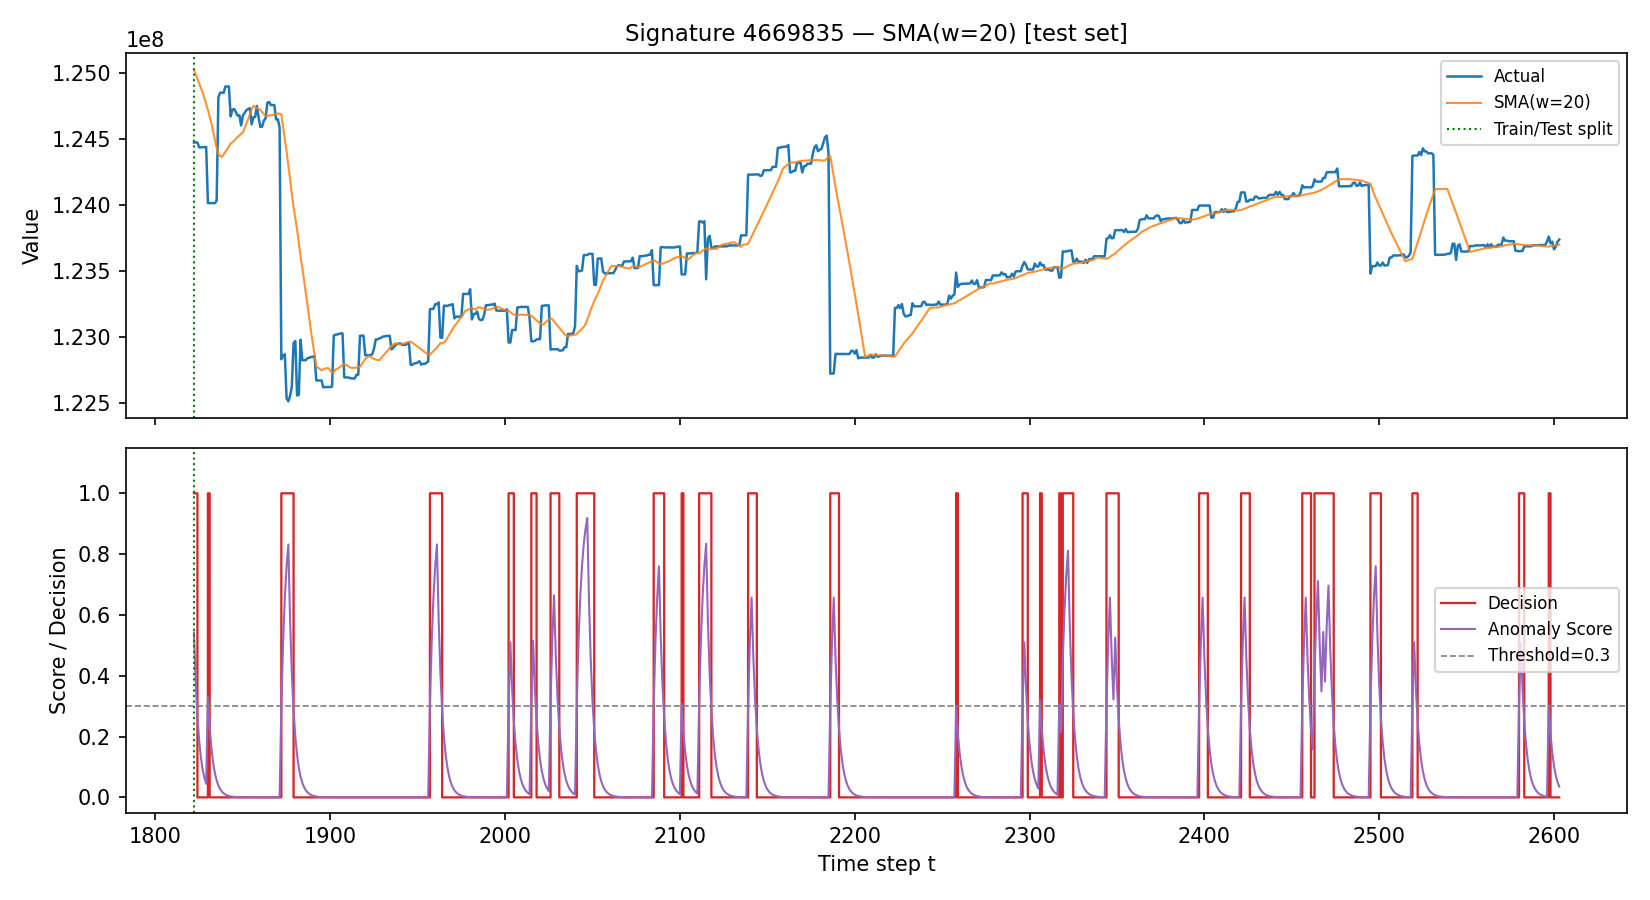
\includegraphics[width=\textwidth]{images/results_plots/4669835_sma.png}
    \caption{SMA(w=20)}
    \label{fig:sample_sma}
  \end{subfigure}
  \hfill
  \begin{subfigure}[t]{0.49\textwidth}
    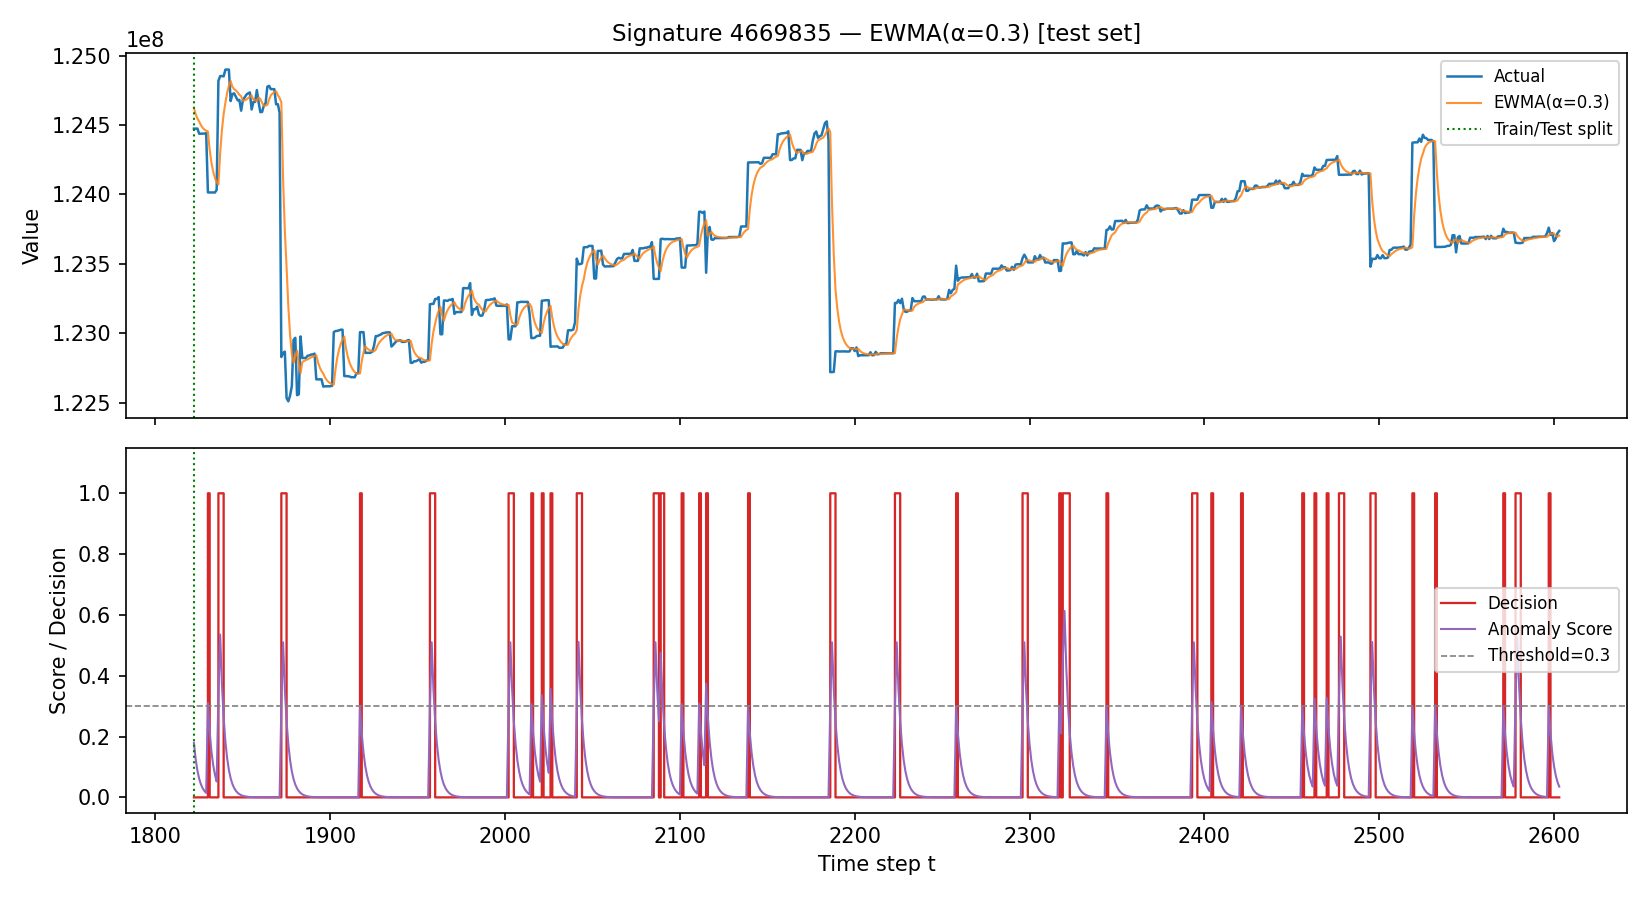
\includegraphics[width=\textwidth]{images/results_plots/4669835_ewma.png}
    \caption{EWMA($\alpha$=0.30)}
    \label{fig:sample_ewma}
  \end{subfigure}
  \caption{Detection output for Mozilla Firefox-Android signature 4669835
    under the four statistical detectors.
    Shaded regions indicate intervals where the detector activated
    tracing ($s_t \geq \theta$). Vertical dashed lines mark ground-truth
    regression alerts.}
  \label{fig:result_sample}
\end{figure*}

\subsection{RQ2: Statistical Significance (Calibration Baseline)}\label{sec:largescale:RQ2}

The following statistical tests are computed on the calibration-baseline
(70\%/30\%, 214-signature) per-signature scores.
The corresponding tests for the canonical 60\%/20\%/20\% test data are
reported separately in Section~\ref{sec:three_way:stats}.

\subsubsection{Bootstrap Confidence Intervals}

Table~\ref{tab:bootstrap_ci} reports 95\% bootstrap confidence intervals
derived from 2,000 resamples with replacement of the 214 calibration-baseline
per-signature scores.

\begin{table}[tbp]
\centering
\resizebox{\columnwidth}{!}{%
\begin{tabular}{lcccc}
\toprule
\textbf{Method} & \textbf{Precision CI} & \textbf{Recall CI} &
  \textbf{F1 CI} & \textbf{FAR CI} \\
\midrule
ARIMA & [0.093,~0.119] & [0.543,~0.668] & [0.154,~0.195] & [0.050,~0.055] \\
LAST  & [0.067,~0.092] & [0.423,~0.550] & [0.114,~0.153] & [0.050,~0.055] \\
SMA   & [0.100,~0.125] & [0.596,~0.719] & [0.166,~0.206] & [0.049,~0.054] \\
EWMA  & [0.078,~0.103] & [0.498,~0.625] & [0.131,~0.171] & [0.053,~0.058] \\
\bottomrule
\end{tabular}%
}
\caption{Bootstrap 95\% confidence intervals (2,000 resamples) on the
  calibration-baseline (214-signature, 70\%/30\%) per-signature scores.}
\label{tab:bootstrap_ci}
\end{table}

The non-overlapping CIs for ARIMA vs.\ LAST (F1: [0.154, 0.195]
vs.\ [0.114, 0.153]) indicate a practically meaningful difference, confirmed
by the Wilcoxon test below.
The CIs for ARIMA and SMA overlap substantially in F1 and precision.

\subsubsection{Wilcoxon Signed-Rank Tests}

Table~\ref{tab:wilcoxon} reports Wilcoxon signed-rank test $p$-values for
all six pairwise comparisons among the four statistical detectors
($\alpha = 0.05$).

\begin{table}[tbp]
\centering
\resizebox{\columnwidth}{!}{%
\begin{tabular}{llcccc}
\toprule
\textbf{Pair} & & \textbf{Precision} & \textbf{Recall} &
  \textbf{F1} & \textbf{FAR} \\
\midrule
ARIMA vs.\ LAST        & $p$ & $<0.001$ & $<0.001$ & $<0.001$ & 0.765$^{*}$ \\
ARIMA vs.\ SMA         & $p$ & 0.652$^{*}$ & 0.001 & 0.547$^{*}$ & 0.380$^{*}$ \\
ARIMA vs.\ EWMA        & $p$ & $<0.001$ & 0.002 & $<0.001$ & $<0.001$ \\
LAST vs.\ SMA          & $p$ & $<0.001$ & $<0.001$ & $<0.001$ & 0.225$^{*}$ \\
LAST vs.\ EWMA         & $p$ & 0.011 & $<0.001$ & 0.006 & 0.013 \\
SMA vs.\ EWMA          & $p$ & $<0.001$ & $<0.001$ & $<0.001$ & $<0.001$ \\
\bottomrule
\multicolumn{6}{l}{\small $^{*}$ Not statistically significant at $\alpha = 0.05$.}
\end{tabular}%
}
\caption{Wilcoxon signed-rank test $p$-values ($n = 214$, calibration baseline)
  for all six pairwise comparisons among the four statistical detectors.
  Cells with $^{*}$ are \emph{not statistically significant} ($p \geq 0.05$).}
\label{tab:wilcoxon}
\end{table}

\textbf{Key findings.}
(i)~ARIMA significantly outperforms LAST on precision, recall, and F1 (all $p<0.001$).
(ii)~ARIMA and SMA do \emph{not} differ significantly in precision ($p=0.652$)
or F1 ($p=0.547$); they differ only in recall ($p=0.001$, SMA higher).
(iii)~ARIMA significantly outperforms EWMA in precision, recall, F1, and FAR (all $p \leq 0.002$).
(iv)~FAR differences between ARIMA and LAST are not significant ($p=0.765$);
LAST vs.\ SMA FAR differences are also not significant ($p=0.225$);
suggesting that ARIMA, LAST, and SMA produce similar false-alarm rates
at this sensitivity setting.

These results answer \textbf{RQ1} (\emph{Among the four statistical methods,
SMA achieves the highest recall (0.657), F1 (0.186), and detection rate (96.0\%),
making it the strongest statistical baseline.
ARIMA is second and statistically indistinguishable from SMA in F1 ($p=0.547$)
and precision ($p=0.652$); LAST is weakest.})
and \textbf{RQ2} (\emph{ARIMA's advantage over LAST and EWMA is statistically
significant in precision, recall, and F1; the ARIMA-vs-SMA difference in F1
and precision is not statistically significant ($p > 0.50$).
All $p<0.001$ cells remain significant under a Bonferroni-corrected threshold
of $\alpha/6 = 0.008$ for the six pairwise comparisons.}).

% ===================================================================
\subsection{Primary Comparative Evaluation: Canonical 60\%/20\%/20\% Protocol}\label{sec:three_way}

This subsection presents the \textbf{canonical results} generated by the
unified pipeline \texttt{run\_full\_evaluation.py}.
All five method families are evaluated on two Mozilla Treeherder repositories
(Section~\ref{sec:largescale:dataset}) under a strict chronological
60\%/20\%/20\% split: Firefox-Android (342 signatures) and mozilla-beta
(1{,}477 signatures).
SMA, EWMA, and Transformer hyperparameters are tuned exclusively on the
held-out validation 20\%; the test 20\% is evaluated exactly once.
\textbf{Readers should treat
Tables~\ref{tab:three_way_fa}--\ref{tab:three_way_mb} as the headline
results of this paper.}

The calibration-baseline results (Section~\ref{sec:largescale:RQ1}) serve
only as a prior-work comparison: they replicate the conference paper's 70/30
setup and are useful for contextualising the ARIMA F1 baseline, but
SMA/EWMA parameters in that evaluation were not independently validated.

\begin{itemize}
  \item \textbf{Train (60\%):} ARIMA parameters are estimated here; all methods
    calibrate their dynamic-threshold $\delta$-history on this portion.
  \item \textbf{Validation (20\%):} SMA~$w$, EWMA~$\alpha$, and Transformer
    hyperparameters (window, $d_{\text{model}}$) are selected by maximising
    mean F1 on this held-out portion independently per dataset.
    ARIMA order~$(1,1,1)$ is kept fixed from the original ablation
    (Section~\ref{sec:ablation}).
    Shared parameters ($\beta=0.30$, $\theta=0.30$) are common to all methods
    and are not tuned on this validation set.
    This is an acknowledged fairness limitation: the ablation study
    (Section~\ref{sec:ablation}) shows that both $\beta$ and $\theta$ exert
    large effects on precision/recall trade-offs, and a per-method or
    per-dataset sweep of these shared parameters might alter the ranking;
    that sweep is left as recommended future work.
  \item \textbf{Test (20\%):} Final metrics are computed on this portion
    exclusively---it was never consulted during any tuning decision.
\end{itemize}

\textbf{Compact Transformer for fair comparison.}
To include a Transformer in the three-way comparison on equal terms, we adopt
a compact architecture (hereafter \emph{Transformer (compact)}):
a single Transformer encoder layer with model dimension $d_{\text{model}}$,
two attention heads, feed-forward dimension $2 d_{\text{model}}$, and a
sliding input window of $w$ samples.
Training uses the Adam optimiser ($\eta=0.01$) with MSE loss, early stopping
(patience~6 on training loss), and a maximum of 20 epochs---the same
Algorithm-3 anomaly-score gating is applied as for all classical detectors
($\beta=0.30$, $\theta=0.30$, $\tau=5$).
This design removes the three adaptive mechanisms (ADT, AnomalyHead, GRAC),
ensuring the only difference from classical methods is the
\emph{forecasting backbone}.
The HP grid sweeps $w \in \{10, 20, 30\}$ and $d_{\text{model}} \in \{8, 16, 32\}$
(nine combinations), tuned with a single seed for efficiency.
The test run uses five independent random seeds $\{42, 123, 456, 789, 1024\}$
and reports mean~$\pm$~standard deviation.

\textbf{Validation-set tuning.}
Figure~\ref{fig:three_way_tuning} shows the validation F1 curves over the
SMA and EWMA grids on both datasets;
Figure~\ref{fig:three_way_transformer_tuning} shows the Transformer HP grid.
\textit{Firefox-Android:} SMA peaks at $w=40$ (val~F1~=~0.102); EWMA peaks
at $\alpha=0.05$ (val~F1~=~0.098); Transformer best at WINDOW=20,
$d_{\text{model}}=16$ (val~F1~=~0.080).
\textit{Mozilla-beta:} SMA peaks at $w=20$ (val~F1~=~0.144); EWMA peaks
at $\alpha=0.05$ (val~F1~=~0.145); Transformer best at WINDOW=10,
$d_{\text{model}}=32$ (val~F1~=~0.130).
SMA curves are unimodal on both datasets with interior optima ($w=40$ and
$w=20$, respectively), confirming that SMA window selection is stable.
The EWMA validation curves also exhibit clear interior optima at $\alpha=0.05$
on both datasets: values below 0.05 (0.01, 0.02, 0.03) all produce lower
validation F1, and values above 0.05 decline monotonically.
This was confirmed by extending the tuning grid to
$\{0.01, 0.02, 0.03, 0.05, 0.10, \ldots, 0.50\}$:
on Firefox-Android the extended grid yields val~F1 values of
0.077, 0.076, 0.088 for $\alpha \in \{0.01, 0.02, 0.03\}$ respectively,
all below the $\alpha=0.05$ peak of 0.098;
on mozilla-beta the pattern is identical
(val~F1~=~0.130, 0.123, 0.135 for $\alpha \in \{0.01, 0.02, 0.03\}$
vs.\ 0.145 at $\alpha=0.05$).
The $\alpha=0.05$ selection is therefore confirmed as an interior optimum
of the full extended grid, not a boundary value.
The optimal Transformer HPs differ across datasets, confirming that
dataset-specific tuning is beneficial.

\begin{figure}[H]
  \centering
  \begin{subfigure}[t]{0.49\textwidth}
    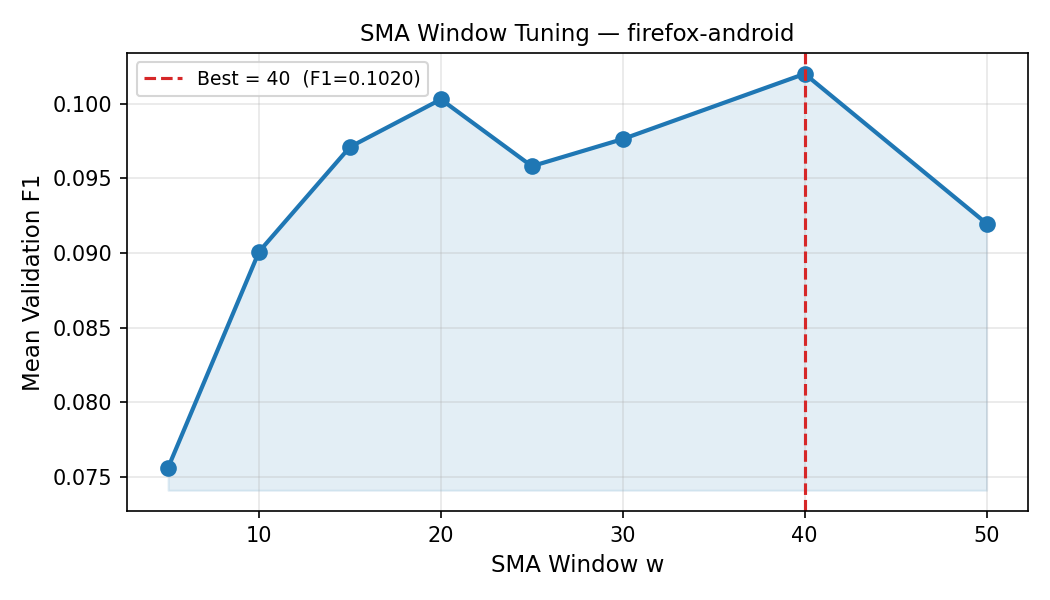
\includegraphics[width=\textwidth]{images/three_way/fa_val_tuning_sma.png}
    \caption{Firefox-Android SMA: peaks at $w=40$.}
    \label{fig:tuning_fa_sma}
  \end{subfigure}
  \hfill
  \begin{subfigure}[t]{0.49\textwidth}
    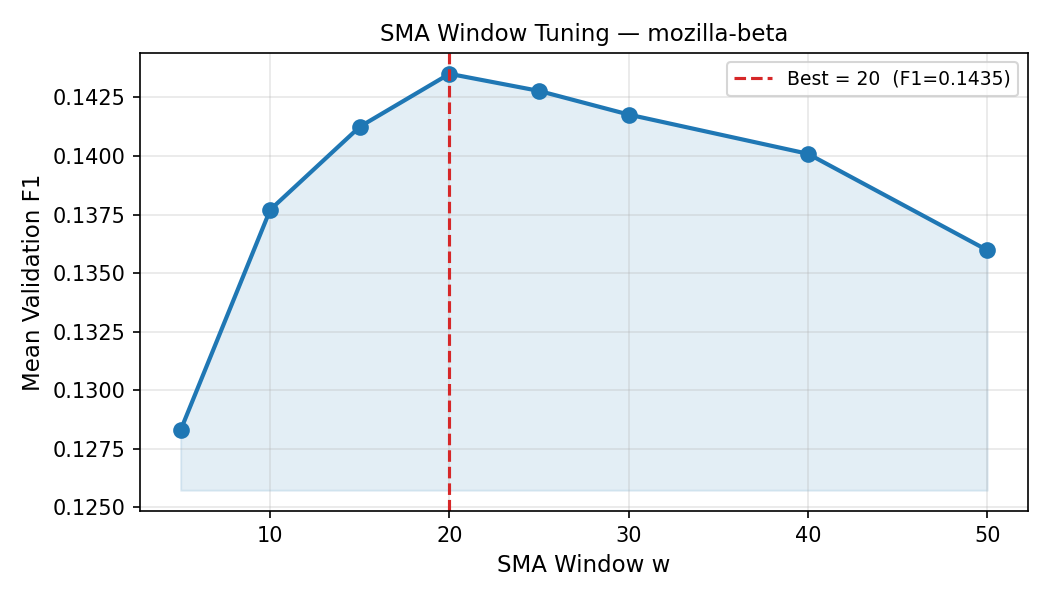
\includegraphics[width=\textwidth]{images/three_way/mb_val_tuning_sma.png}
    \caption{mozilla-beta SMA: peaks at $w=20$.}
    \label{fig:tuning_mb_sma}
  \end{subfigure}
  \\[6pt]
  \begin{subfigure}[t]{0.49\textwidth}
    
\includegraphics[width=\textwidth]{images/three_way/fa_val_tuning_ewma_extended.png}
    \caption{Firefox-Android EWMA: peaks at $\alpha=0.05$ (interior optimum confirmed by extended grid down to $\alpha=0.01$).}
    \label{fig:tuning_fa_ewma}
  \end{subfigure}
  \hfill
  \begin{subfigure}[t]{0.49\textwidth}
    
\includegraphics[width=\textwidth]{images/three_way/mb_val_tuning_ewma_extended.png}
    \caption{mozilla-beta EWMA: peaks at $\alpha=0.05$ (interior optimum confirmed by extended grid down to $\alpha=0.01$).}
    \label{fig:tuning_mb_ewma}
  \end{subfigure}
  \caption{Validation-set parameter tuning curves for SMA (top row) and EWMA
    (bottom row) on Firefox-Android (left) and mozilla-beta (right).
    Red dashed lines mark the selected parameter value.
    SMA curves are unimodal with interior optima, confirming stable window
    selection.
    EWMA curves also exhibit clear interior optima at $\alpha=0.05$ on both
    datasets: an extended grid down to $\alpha=0.01$ confirms that smaller
    values reduce validation F1, so $\alpha=0.05$ is a confirmed interior
    optimum, not a grid boundary.}
  \label{fig:three_way_tuning}
\end{figure}

\begin{figure}[H]
  \centering
  \begin{subfigure}[t]{0.49\textwidth}
    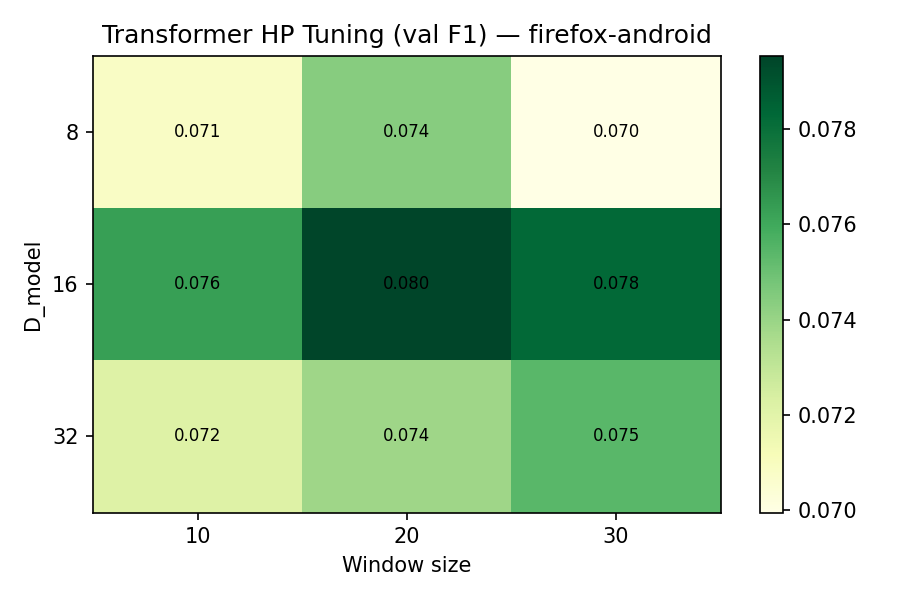
\includegraphics[width=\textwidth]{images/three_way/fa_val_tuning_transformer.png}
    \caption{Firefox-Android: best WINDOW=20, $d_{\text{model}}=16$.}
    \label{fig:tuning_fa_transformer}
  \end{subfigure}
  \hfill
  \begin{subfigure}[t]{0.49\textwidth}
    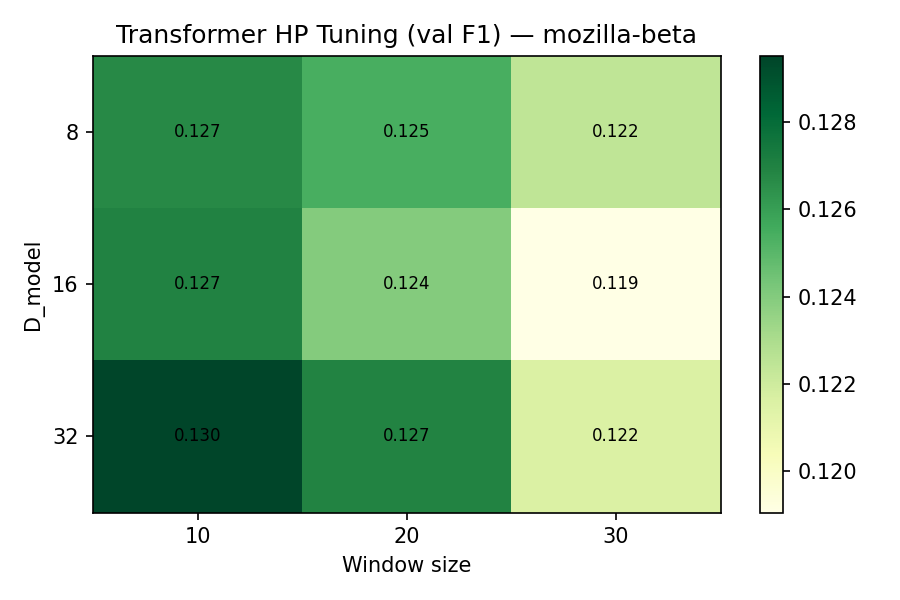
\includegraphics[width=\textwidth]{images/three_way/mb_val_tuning_transformer.png}
    \caption{mozilla-beta: best WINDOW=10, $d_{\text{model}}=32$.}
    \label{fig:tuning_mb_transformer}
  \end{subfigure}
  \caption{Compact Transformer HP validation F1 over the
    $\{10,20,30\} \times \{8,16,32\}$ window $\times$ $d_{\text{model}}$ grid
    (single-seed tuning run).
    Different optimal HPs per dataset indicate the benefit of per-dataset tuning.}
  \label{fig:three_way_transformer_tuning}
\end{figure}

\textbf{Test-set results.}
Tables~\ref{tab:three_way_fa} and~\ref{tab:three_way_mb} report the final
test-set metrics for all five method families.
The 20\% test window contains 136 of 342 (39.8\%) Firefox-Android signatures
and 395 of 1{,}477 (26.7\%) mozilla-beta signatures with $\geq 1$ alert.

\begin{table}[tbp]
\centering
\resizebox{\columnwidth}{!}{%
\begin{tabular}{lcccccc}
\toprule
\textbf{Method} & \textbf{Precision} & \textbf{Recall} & \textbf{F1} &
  \textbf{FAR} & \textbf{Det.\ Rate (\%)} & \textbf{Storage Red.\ (\%)} \\
\midrule
ARIMA(1,1,1)                     & 0.056 & 0.257 & 0.089 & 0.056 & 66.18 & 90.30 \\
LAST                             & 0.046 & 0.209 & 0.072 & 0.055 & 54.41 & 89.15 \\
SMA($w=40$)$^\dagger$            & 0.066 & \textbf{0.290} & \textbf{0.104} & 0.055 & \textbf{72.79} & 88.26 \\
EWMA($\alpha$=0.05)$^\dagger$    & \textbf{0.068} & 0.263 & 0.103 & \textbf{0.052} & 67.65 & \textbf{89.43} \\
Transformer (compact)$^\ddagger$ & 0.069 {\small $\pm$0.002} &
  0.292 {\small $\pm$0.002} & 0.105 {\small $\pm$0.002} &
  0.066 {\small $\pm$0.001} & 74.41 & 67.21 \\
\bottomrule
\end{tabular}%
}
\caption{Three-way split (60\%/20\%/20\%) test-set results on
  \textbf{Firefox-Android} (342 signatures; 136 with $\geq 1$ alert in
  the test set).
  $^\dagger$ parameter tuned on the held-out validation set.
  $^\ddagger$ Transformer (compact): $d_{\text{model}}=16$, WINDOW=20,
  one encoder layer, MSE+Adam (no ADT/Ano\-malyHead/GRAC);
  five seeds, mean~$\pm$~std.
  Bold marks the best value per column among classical statistical methods
  (Transformer excluded from bold).}
\label{tab:three_way_fa}
\end{table}

\begin{table}[tbp]
\centering
\resizebox{\columnwidth}{!}{%
\begin{tabular}{lcccccc}
\toprule
\textbf{Method} & \textbf{Precision} & \textbf{Recall} & \textbf{F1} &
  \textbf{FAR} & \textbf{Det.\ Rate (\%)} & \textbf{Storage Red.\ (\%)} \\
\midrule
ARIMA(1,1,1)                     & 0.050 & 0.232 & 0.076 & 0.060 & 88.61 & 90.31 \\
LAST                             & 0.045 & 0.212 & 0.069 & \textbf{0.053} & 81.77 & 89.03 \\
SMA($w=20$)$^\dagger$            & \textbf{0.057} & \textbf{0.241} & \textbf{0.085} & 0.059 & \textbf{91.65} & 88.84 \\
EWMA($\alpha$=0.05)$^\dagger$    & 0.057 & 0.236 & 0.083 & 0.059 & 90.63 & \textbf{88.47} \\
Transformer (compact)$^\ddagger$ & 0.054 {\small $\pm$0.001} &
  0.235 {\small $\pm$0.002} & 0.079 {\small $\pm$0.001} &
  0.064 {\small $\pm$0.000} & 89.82 & 71.09 \\
\bottomrule
\end{tabular}%
}
\caption{Three-way split (60\%/20\%/20\%) test-set results on
  \textbf{mozilla-beta} (1{,}477 signatures; 395 with $\geq 1$ alert in
  the test set).
  $^\dagger$ parameter tuned on the held-out validation set.
  $^\ddagger$ Transformer (compact): $d_{\text{model}}=32$, WINDOW=10,
  one encoder layer, MSE+Adam (no ADT/Ano\-malyHead/GRAC);
  five seeds, mean~$\pm$~std.
  Bold marks the best value per column among classical statistical methods
  (Transformer excluded from bold).}
\label{tab:three_way_mb}
\end{table}

Six findings emerge from Tables~\ref{tab:three_way_fa}--\ref{tab:three_way_mb}:

\begin{enumerate}
  \item \textbf{Qualitative ranking is consistent across both datasets.}
    SMA and EWMA lead on most accuracy dimensions; ARIMA is third; LAST
    is weakest among the statistical methods on both Firefox-Android and
    mozilla-beta.
    The directional conclusions of the main evaluation are robust to proper
    hold-out parameter selection and generalise to a second dataset.

  \item \textbf{EWMA at $\alpha=0.05$ matches SMA in F1; the optimum is confirmed by an extended grid.}
    Under independent per-dataset tuning, EWMA achieves F1~=~0.103
    (Firefox-Android) and F1~=~0.083 (mozilla-beta)---within 0.001--0.002
    of the corresponding SMA F1 on both datasets.
    Both datasets select $\alpha=0.05$.
    An extended tuning grid covering $\{0.01, 0.02, 0.03, 0.05, 0.10,
    \ldots, 0.50\}$ was evaluated; on Firefox-Android, val~F1 values for
    $\alpha \in \{0.01, 0.02, 0.03\}$ are 0.077, 0.076, and 0.088
    respectively---all below the $\alpha=0.05$ peak of 0.098.
    On mozilla-beta the same pattern holds
    (0.130, 0.123, 0.135 vs.\ 0.145 at $\alpha=0.05$).
    The $\alpha=0.05$ selection is therefore a confirmed interior optimum,
    and the test-set results are unchanged.
    EWMA achieves higher storage reduction than SMA on Firefox-Android
    (89.4\% vs.\ 88.3\%); on mozilla-beta the margin reverses slightly
    (EWMA 88.5\% vs.\ SMA 88.8\%), so the storage advantage is
    Firefox-Android-specific rather than a consistent cross-dataset finding.
    On Firefox-Android, EWMA is attractive when storage efficiency is a
    priority alongside competitive detection quality.

  \item \textbf{ARIMA outperforms LAST on both datasets.}
    Firefox-Android: detection rate 66.2\% vs.\ 54.4\%; F1~0.089 vs.\ 0.072.
    Mozilla-beta: detection rate 88.6\% vs.\ 81.8\%; F1~0.076 vs.\ 0.069.
    The ARIMA advantage established in the main evaluation carries through
    to both the 60/20/20 split and the second dataset.

  \item \textbf{Compact Transformer is competitive with top classical methods
    on Firefox-Android.}
    On Firefox-Android, the compact Transformer achieves
    F1~=~0.105~($\pm$0.002), marginally above SMA F1~=~0.104, with
    detection rate 74.4\% exceeding SMA (72.8\%).
    Standard deviation across five seeds is $\leq$0.002 for all metrics,
    confirming that training variability is not a confound.

  \item \textbf{Compact Transformer falls slightly below classical methods
    on mozilla-beta.}
    On the larger mozilla-beta dataset, the compact Transformer achieves
    F1~=~0.079~($\pm$0.001), below SMA F1~=~0.085 ($-$0.006) and
    EWMA F1~=~0.083 ($-$0.004).
    Seed stability remains high (std $\leq$0.001), indicating the result
    is consistent across training runs.

  \item \textbf{Storage reduction differs by predictor type.}
    Classical methods achieve 88--90\% storage reduction on both datasets.
    The compact Transformer achieves 67.2\% (Firefox-Android) and 71.1\%
    (mozilla-beta)---lower because the learned predictor activates
    trace-on windows more frequently at the same anomaly-score threshold.
    Practitioners prioritising storage savings should consider threshold
    adjustment for Transformer-based deployment.
\end{enumerate}

Figure~\ref{fig:three_way_comparison} shows the test-set metrics for all five
methods across both datasets.

\begin{figure}[H]
  \centering
  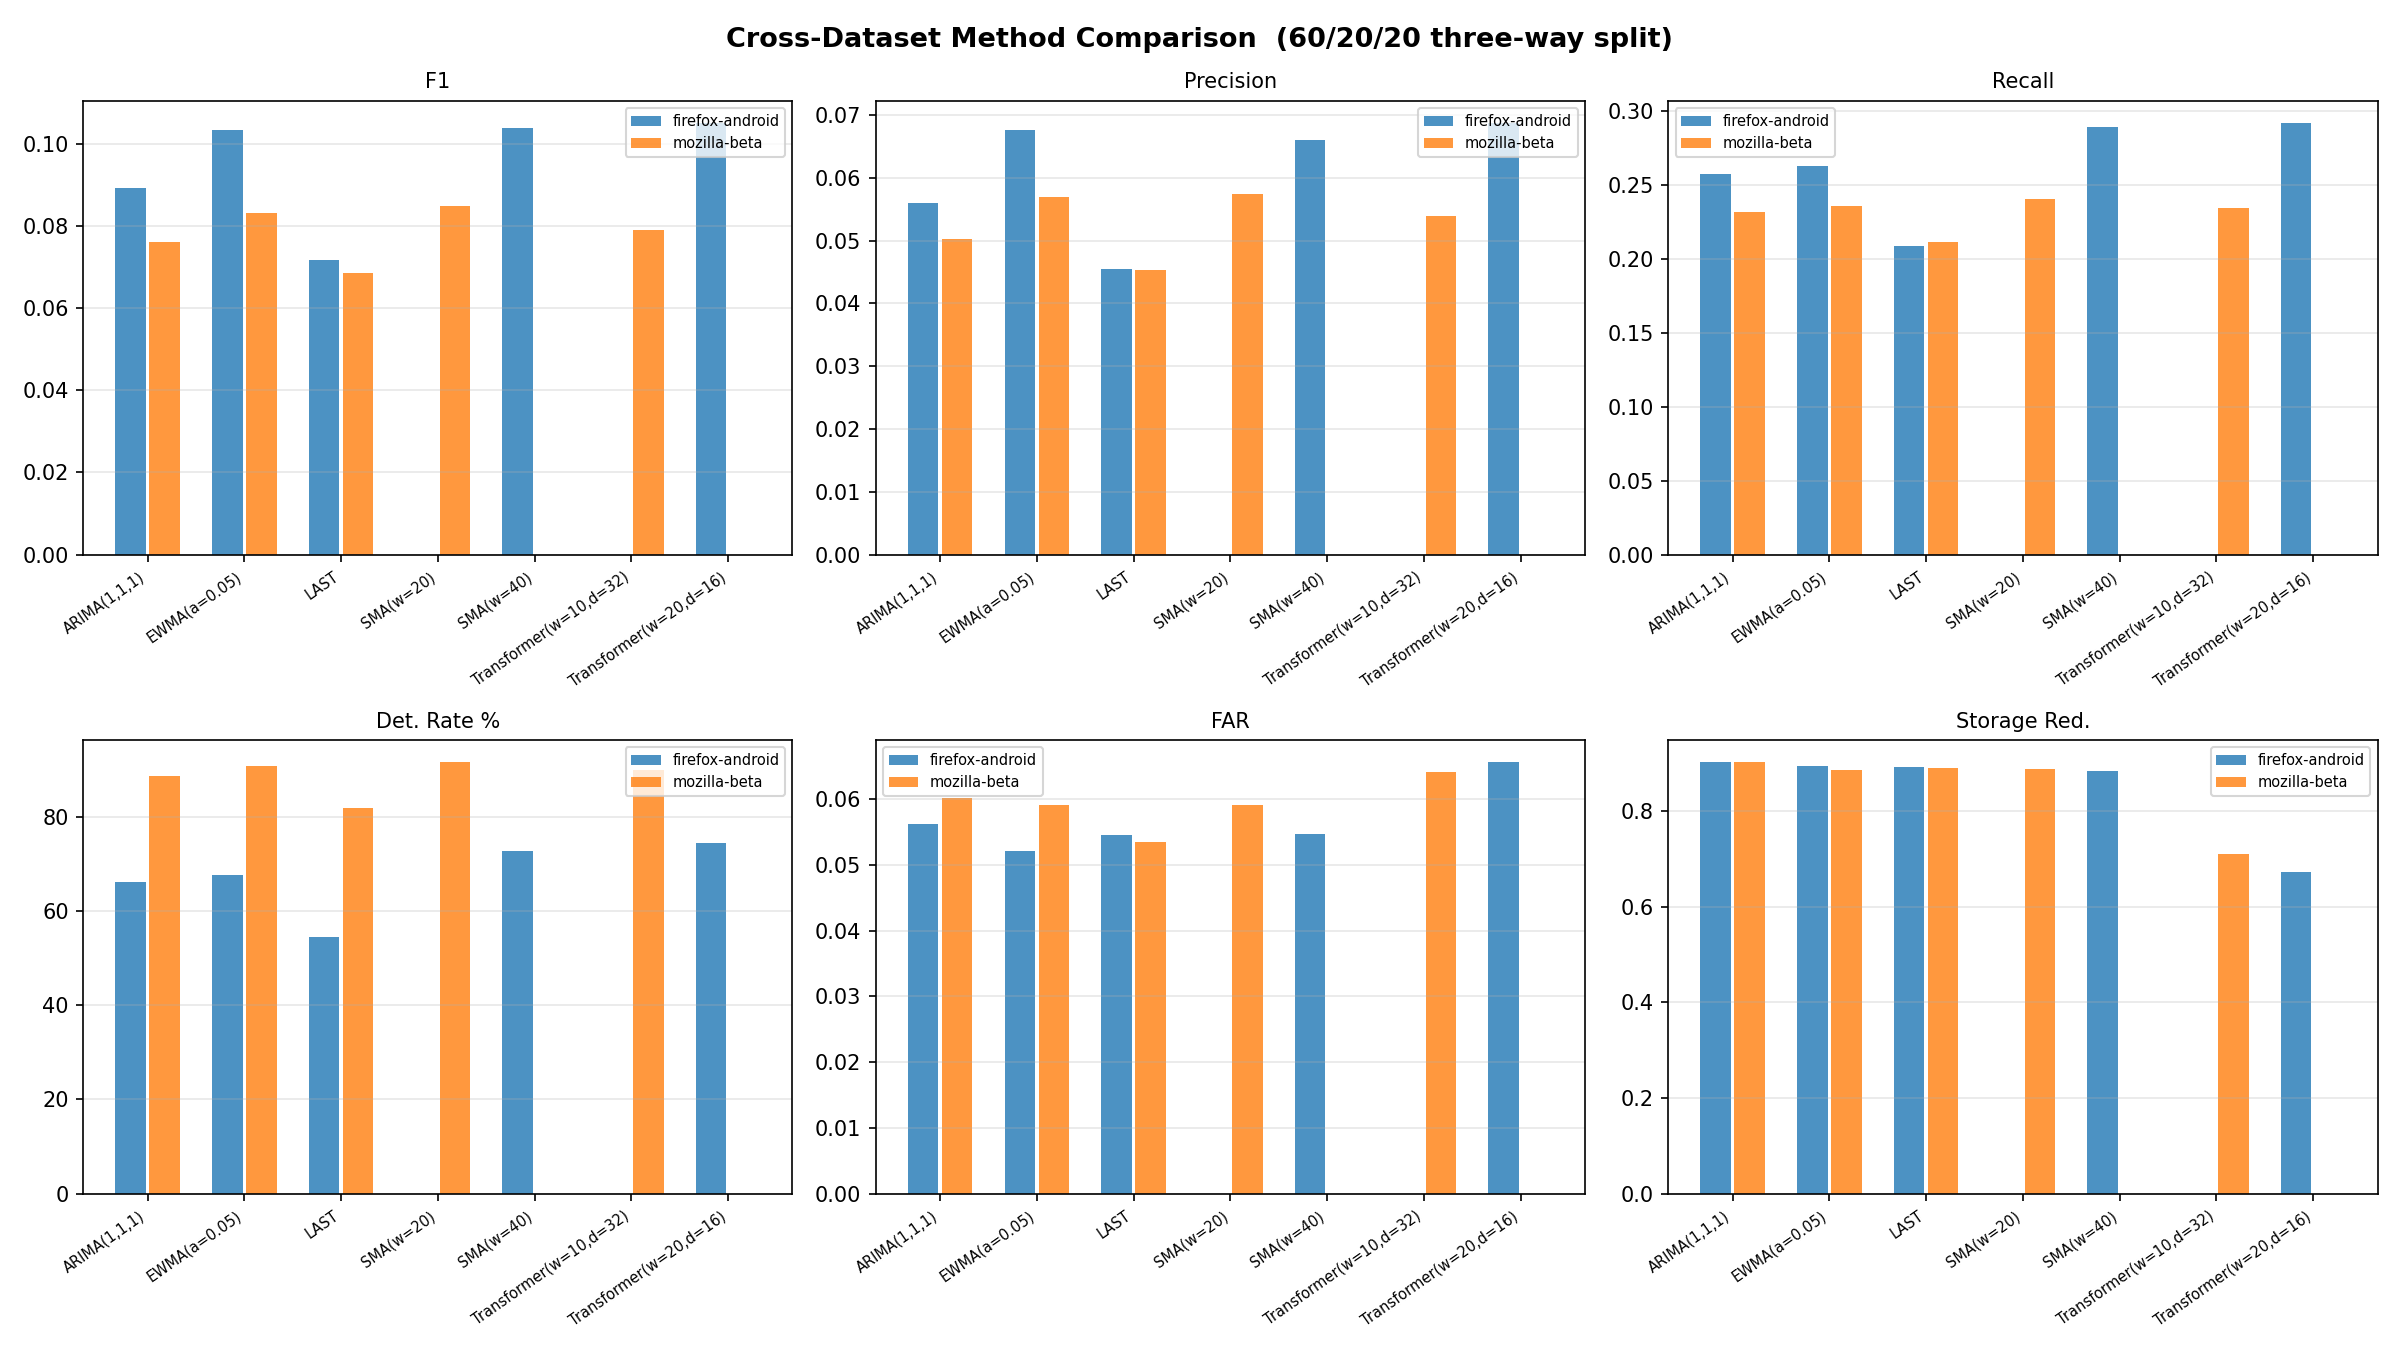
\includegraphics[width=\linewidth]{images/combined_comparison.png}
  \caption{Test-set metrics for all five methods on both datasets under the
    60\%/20\%/20\% three-way split.
    The qualitative ranking
    SMA~$\approx$~EWMA~$\geq$~ARIMA~$>$~LAST is consistent across datasets.}
  \label{fig:three_way_comparison}
\end{figure}

% -------------------------------------------------------------------
\subsection{Statistical Significance: Canonical 60\%/20\%/20\% Protocol}\label{sec:three_way:stats}
% -------------------------------------------------------------------

This subsection provides inferential support for the headline results in
Tables~\ref{tab:three_way_fa}--\ref{tab:three_way_mb}.
Bootstrap confidence intervals and Wilcoxon signed-rank tests are computed
directly on the 342 (Firefox-Android) and 1{,}477 (mozilla-beta)
per-signature test-set scores produced by the canonical pipeline.
The Bonferroni-corrected significance threshold for six pairwise comparisons
among the four statistical methods is $\alpha/6 = 0.0083$; cells
below this threshold are marked with $^{*}$ in the tables.

\subsubsection{Bootstrap Confidence Intervals}

Tables~\ref{tab:can_ci_fa} and~\ref{tab:can_ci_mb} report 95\% bootstrap
confidence intervals (2{,}000 resamples) on the canonical per-signature
test-set scores.

\begin{table}[tbp]
\centering
\resizebox{\columnwidth}{!}{%
\begin{tabular}{lcccc}
\toprule
\textbf{Method} & \textbf{Precision CI} & \textbf{Recall CI} &
  \textbf{F1 CI} & \textbf{FAR CI} \\
\midrule
ARIMA & [0.045,~0.068] & [0.212,~0.307] & [0.072,~0.107] & [0.054,~0.059] \\
LAST  & [0.035,~0.057] & [0.168,~0.254] & [0.057,~0.087] & [0.053,~0.057] \\
SMA   & [0.054,~0.079] & [0.243,~0.336] & [0.086,~0.123] & [0.052,~0.057] \\
EWMA  & [0.054,~0.081] & [0.218,~0.311] & [0.084,~0.124] & [0.050,~0.055] \\
\bottomrule
\end{tabular}%
}
\caption{Bootstrap 95\% confidence intervals (2{,}000 resamples) on the
  canonical (60\%/20\%/20\%, $n=342$ signatures) per-signature test-set
  scores for Firefox-Android.}
\label{tab:can_ci_fa}
\end{table}

\begin{table}[tbp]
\centering
\resizebox{\columnwidth}{!}{%
\begin{tabular}{lcccc}
\toprule
\textbf{Method} & \textbf{Precision CI} & \textbf{Recall CI} &
  \textbf{F1 CI} & \textbf{FAR CI} \\
\midrule
ARIMA & [0.044,~0.057] & [0.211,~0.254] & [0.068,~0.084] & [0.059,~0.061] \\
LAST  & [0.039,~0.052] & [0.191,~0.231] & [0.061,~0.076] & [0.053,~0.054] \\
SMA   & [0.050,~0.065] & [0.220,~0.263] & [0.076,~0.095] & [0.058,~0.060] \\
EWMA  & [0.050,~0.064] & [0.215,~0.259] & [0.074,~0.092] & [0.058,~0.060] \\
\bottomrule
\end{tabular}%
}
\caption{Bootstrap 95\% confidence intervals (2{,}000 resamples) on the
  canonical (60\%/20\%/20\%, $n=1{,}477$ signatures) per-signature test-set
  scores for mozilla-beta.}
\label{tab:can_ci_mb}
\end{table}

Key observations from the CIs:
\begin{itemize}
  \item On Firefox-Android, SMA and EWMA F1 intervals overlap substantially
    ([0.086,~0.123] and [0.084,~0.124]), confirming the near-tie in
    Table~\ref{tab:three_way_fa}.
  \item LAST F1 interval ([0.057,~0.087] on Firefox-Android;
    [0.061,~0.076] on mozilla-beta) is non-overlapping with SMA and EWMA
    on both datasets, indicating a practically meaningful gap.
  \item On mozilla-beta, SMA and EWMA F1 intervals again overlap
    ([0.076,~0.095] vs.\ [0.074,~0.092]), consistent with the
    near-tie in Table~\ref{tab:three_way_mb}.
\end{itemize}

\subsubsection{Wilcoxon Signed-Rank Tests}

Tables~\ref{tab:can_wil_fa} and~\ref{tab:can_wil_mb} report Wilcoxon
signed-rank test $p$-values for all six pairwise comparisons on the
canonical test-set scores ($n=342$ and $n=1{,}477$ respectively).

\begin{table}[tbp]
\centering
\resizebox{\columnwidth}{!}{%
\begin{tabular}{llcccc}
\toprule
\textbf{Pair} & & \textbf{Precision} & \textbf{Recall} &
  \textbf{F1} & \textbf{FAR} \\
\midrule
ARIMA vs.\ LAST        & $p$ & $<0.001^{*}$ & $<0.001^{*}$ & $<0.001^{*}$ & 0.107$^{\dag}$ \\
ARIMA vs.\ SMA         & $p$ & 0.006$^{*}$  & 0.006$^{*}$  & 0.004$^{*}$  & 0.084$^{\dag}$ \\
ARIMA vs.\ EWMA        & $p$ & $<0.001^{*}$ & 0.482$^{\dag}$ & $<0.001^{*}$ & $<0.001^{*}$ \\
LAST vs.\ SMA          & $p$ & $<0.001^{*}$ & $<0.001^{*}$ & $<0.001^{*}$ & 0.969$^{\dag}$ \\
LAST vs.\ EWMA         & $p$ & $<0.001^{*}$ & $<0.001^{*}$ & $<0.001^{*}$ & 0.060$^{\dag}$ \\
SMA vs.\ EWMA          & $p$ & 0.729$^{\dag}$ & 0.017$^{*}$  & 0.965$^{\dag}$ & $<0.001^{*}$ \\
\bottomrule
\multicolumn{6}{l}{\small $^{*}$ Significant at Bonferroni-corrected $\alpha/6=0.0083$.
  $^{\dag}$ Not significant.}
\end{tabular}%
}
\caption{Wilcoxon signed-rank $p$-values on the canonical
  60\%/20\%/20\% test set, Firefox-Android ($n=342$ signatures).}
\label{tab:can_wil_fa}
\end{table}

\begin{table}[tbp]
\centering
\resizebox{\columnwidth}{!}{%
\begin{tabular}{llcccc}
\toprule
\textbf{Pair} & & \textbf{Precision} & \textbf{Recall} &
  \textbf{F1} & \textbf{FAR} \\
\midrule
ARIMA vs.\ LAST        & $p$ & $<0.001^{*}$ & $<0.001^{*}$ & $<0.001^{*}$ & $<0.001^{*}$ \\
ARIMA vs.\ SMA         & $p$ & $<0.001^{*}$ & 0.006$^{*}$  & $<0.001^{*}$ & 0.005$^{*}$ \\
ARIMA vs.\ EWMA        & $p$ & $<0.001^{*}$ & 0.100$^{\dag}$ & $<0.001^{*}$ & 0.003$^{*}$ \\
LAST vs.\ SMA          & $p$ & $<0.001^{*}$ & $<0.001^{*}$ & $<0.001^{*}$ & $<0.001^{*}$ \\
LAST vs.\ EWMA         & $p$ & $<0.001^{*}$ & $<0.001^{*}$ & $<0.001^{*}$ & $<0.001^{*}$ \\
SMA vs.\ EWMA          & $p$ & 0.124$^{\dag}$ & 0.069$^{\dag}$ & 0.102$^{\dag}$ & 0.855$^{\dag}$ \\
\bottomrule
\multicolumn{6}{l}{\small $^{*}$ Significant at Bonferroni-corrected $\alpha/6=0.0083$.
  $^{\dag}$ Not significant.}
\end{tabular}%
}
\caption{Wilcoxon signed-rank $p$-values on the canonical
  60\%/20\%/20\% test set, mozilla-beta ($n=1{,}477$ signatures).}
\label{tab:can_wil_mb}
\end{table}

\textbf{Key findings from the canonical statistical tests.}
(i)~ARIMA significantly outperforms LAST on every metric for both datasets
(all $p < 0.001$).
(ii)~On Firefox-Android, ARIMA is statistically inferior to SMA in
precision, recall, and F1 (all $p \leq 0.006$), unlike the calibration
baseline where the ARIMA--SMA F1 gap was not significant.
This reflects the smaller canonical training proportion (60\% vs.\ 70\%),
benefiting the parameter-free SMA.
(iii)~SMA and EWMA are \emph{not} significantly different in precision
or F1 on either dataset ($p \geq 0.10$), confirming the near-tie in
Tables~\ref{tab:three_way_fa}--\ref{tab:three_way_mb}.
(iv)~On mozilla-beta, ARIMA is significantly worse than both SMA and EWMA
in F1 (both $p < 0.001$), strengthening the case that SMA and EWMA
are the preferred canonical choices.
(v)~LAST is significantly inferior to SMA and EWMA on both datasets
in precision, recall, and F1 (all $p < 0.001$).
(vi)~EWMA achieves significantly lower FAR than SMA on Firefox-Android
($p < 0.001$), reflecting its more conservative activation policy.

% ===================================================================
\section{Ablation Study}\label{sec:ablation}
% ===================================================================

\noindent\fbox{\parbox{\columnwidth}{\small
\textbf{Ground-truth definition.}
The ablation tables use a \emph{stricter} ground truth than the main
calibration-baseline table (Table~\ref{tab:main_results}): only
\emph{regression-classified} Treeherder alerts are counted as positives,
whereas the main table counts all Treeherder alerts.
Because the regression subset is a strict subset of all alerts,
ablation precision, recall, and F1 values at every operating point are
lower than their main-table counterparts.
Specifically, at the shared default ($\beta=0.30$, $\theta=0.30$, $\tau=5$)
ARIMA yields F1~=~0.174 under the main-table GT and F1~=~0.144 under
the stricter ablation GT; SMA yields F1~=~0.186 vs.\ 0.155, respectively.
This gap is intentional: the stricter GT isolates parameter sensitivity
from the effect of borderline alerts, giving a cleaner sweep signal.
All \emph{relative} comparisons within each ablation table are unaffected.
}}

\medskip
To address \textbf{RQ3} we sweep the five most influential parameters and
report effects on mean precision, recall, F1, and FAR.
All ablations use ARIMA(1,1,1) as the primary method, with SMA included
for the $\tau$ sweep.
The four statistical detectors therefore provide the primary ablation signal.

\subsection{Decay Factor \texorpdfstring{$\beta$}{beta}}\label{sec:ablation:beta}

Table~\ref{tab:ablation_beta} shows results for $\beta \in \{0.1, 0.2, 0.3,
0.5, 0.7\}$.

\begin{table}[tbp]
\centering
\begin{tabular}{ccccc}
\toprule
$\beta$ & Precision & Recall & F1 & FAR \\
\midrule
0.10 & 0.173 & 0.210 & 0.183 & 0.003 \\
0.20 & 0.204 & 0.479 & 0.266 & 0.018 \\
\textbf{0.30} & \textbf{0.086} & \textbf{0.544} & \textbf{0.144} & \textbf{0.054} \\
0.50 & 0.086 & 0.540 & 0.144 & 0.055 \\
0.70 & 0.082 & 0.502 & 0.137 & 0.057 \\
\bottomrule
\end{tabular}
\caption{Effect of $\beta$ on ARIMA(1,1,1) detection performance
  (ablation GT: regression-classified alerts only; see section header note).
  Bold marks the chosen default ($\beta = 0.30$).
  At this default, the main-table GT yields F1~=~0.174 (Table~\ref{tab:main_results}).}
\label{tab:ablation_beta}
\end{table}

Smaller $\beta$ values (0.1, 0.2) produce markedly higher precision and F1
for ARIMA (F1~=~0.266 at $\beta=0.20$ vs.\ 0.144 at the default $\beta=0.30$
under the ablation GT; the corresponding main-table GT value at the default
is F1~=~0.174, see Table~\ref{tab:main_results}),
because the score accumulates more selectively.
However, ARIMA recall drops substantially (0.479 at $\beta=0.20$ vs.~0.544 at $\beta=0.30$)
because the score rises too slowly to cross the threshold before the alert window
closes.
Large $\beta$ values ($\geq 0.50$) increase FAR because isolated spikes more readily push
the score above threshold; ARIMA F1 stabilises at $\approx$0.14 for $\beta \geq 0.50$
while recall continues to decline (0.540 at $\beta=0.50$ to 0.502 at $\beta=0.70$).
The default $\beta = 0.30$ was retained as an operational tradeoff: it achieves
high recall and responds more reliably to sustained anomalies in deployment
scenarios where missing a regression is costlier than a false alarm.
Practitioners optimising for F1 rather than recall should note that
$\beta = 0.20$ (ARIMA: F1~=~0.266) yields demonstrably better F1 on this benchmark.

\subsection{Anomaly-Score Threshold \texorpdfstring{$\theta$}{theta}}\label{sec:ablation:threshold}

Table~\ref{tab:ablation_threshold} sweeps $\theta \in \{0.10, 0.15, 0.20, 0.25,
0.30, 0.40, 0.50\}$.

\begin{table}[tbp]
\centering
\begin{tabular}{ccccc}
\toprule
$\theta$ & Precision & Recall & F1 & FAR \\
\midrule
0.10 & 0.097 & 0.591 & 0.162 & 0.042 \\
0.15 & 0.097 & 0.591 & 0.162 & 0.047 \\
0.20 & 0.095 & 0.591 & 0.160 & 0.049 \\
0.25 & 0.091 & 0.591 & 0.154 & 0.053 \\
\textbf{0.30} & \textbf{0.086} & \textbf{0.544} & \textbf{0.144} & \textbf{0.054} \\
0.40 & 0.214 & 0.465 & 0.272 & 0.017 \\
0.50 & 0.227 & 0.402 & 0.270 & 0.011 \\
\bottomrule
\end{tabular}
\caption{Effect of anomaly-score threshold $\theta$ on ARIMA(1,1,1) performance
  (ablation GT: regression-classified alerts only; see section header note).
  Bold marks the default ($\theta = 0.30$).}
\label{tab:ablation_threshold}
\end{table}

For ARIMA, F1 is marginally higher at $\theta \in [0.10, 0.25]$
(up to 0.162 vs.\ 0.144 at the default, both under the ablation GT).
Above $\theta = 0.30$ the behaviour bifurcates:
ARIMA sees a large precision jump and recall drop, with F1 rising substantially:
F1~=~0.272 at $\theta=0.40$ (precision 0.214, recall 0.465) and
F1~=~0.270 at $\theta=0.50$ (precision 0.227, recall 0.402).
These high-$\theta$ operating points trade recall for precision and F1;
the higher F1 arises because only the strongest, most sustained anomaly
episodes cross the threshold, dramatically reducing false-alarm intervals.
The default $\theta = 0.30$ was chosen as a high-recall operating point;
practitioners targeting precision-oriented F1 over recall should consider
$\theta = 0.40$--$0.50$ for ARIMA.

\subsection{Tolerance Window \texorpdfstring{$\tau$}{tau}}\label{sec:ablation:tau}

Table~\ref{tab:ablation_tau} shows results for $\tau \in \{1, 2, 3, 5, 7, 10\}$.

\begin{table}[tbp]
\centering
\begin{tabular}{clcccc}
\toprule
$\tau$ & Method & Precision & Recall & F1 & FAR \\
\midrule
\multirow{2}{*}{1}  & ARIMA & 0.049 & 0.423 & 0.087 & 0.056 \\
                    & SMA   & 0.057 & 0.470 & 0.100 & 0.055 \\
\multirow{2}{*}{3}  & ARIMA & 0.064 & 0.474 & 0.110 & 0.055 \\
                    & SMA   & 0.071 & 0.535 & 0.123 & 0.054 \\
\multirow{2}{*}{\textbf{5}}  & \textbf{ARIMA} & \textbf{0.086} & \textbf{0.544} & \textbf{0.144} & \textbf{0.054} \\
                    & \textbf{SMA}   & \textbf{0.092} & \textbf{0.591} & \textbf{0.155} & \textbf{0.053} \\
\multirow{2}{*}{7}  & ARIMA & 0.103 & 0.591 & 0.171 & 0.053 \\
                    & SMA   & 0.099 & 0.591 & 0.166 & 0.053 \\
\multirow{2}{*}{10} & ARIMA & 0.115 & 0.591 & 0.187 & 0.052 \\
                    & SMA   & 0.109 & 0.591 & 0.179 & 0.052 \\
\bottomrule
\end{tabular}
\caption{Effect of tolerance $\tau$ (samples) on ARIMA and SMA.
  Bold marks the default ($\tau = 5$).}
\label{tab:ablation_tau}
\end{table}

Metrics improve monotonically with $\tau$ for both methods because more
alert--detection matchings are permitted; all methods plateau around $\tau = 7$,
suggesting that a 5-sample neighbourhood captures most valid detections without
inflating scores artificially.

\subsection{ARIMA Order}\label{sec:ablation:order}

Table~\ref{tab:ablation_order} compares five ARIMA configurations on a
stratified 50-signature subset (every $N$th series drawn from the
length-sorted pool of 214 Firefox-Android signals, using a 70\%/30\%
chronological split and the same pipeline parameters as the main evaluation).
Results are reported as means over the 50 signatures.

\begin{table}[tbp]
\centering
\begin{tabular}{lcccc}
\toprule
Order & Precision & Recall & F1 & FAR \\
\midrule
(1,0,0) & 0.033 & 0.300 & 0.058 & 0.072 \\
(0,1,1) & 0.039 & 0.280 & 0.067 & 0.063 \\
(1,1,0) & 0.037 & 0.300 & 0.065 & 0.063 \\
\textbf{(1,1,1)} & \textbf{0.039} & \textbf{0.280} & \textbf{0.067} & \textbf{0.063} \\
(2,1,2) & 0.038 & 0.280 & 0.066 & 0.062 \\
\bottomrule
\end{tabular}
\caption{ARIMA order ablation (50-signature stratified subset,
  70\%/30\% split, same pipeline as main evaluation).
  Bold marks the chosen default.
  Results are indicative of relative order performance within this subset;
  strong generalisation claims across the full benchmark are not warranted.}
\label{tab:ablation_order}
\end{table}

On the expanded 50-signature subset, all integrated-difference models
((0,1,1), (1,1,0), (1,1,1), (2,1,2)) produce essentially equivalent
F1 scores within a range of 0.001 (0.065--0.067),
substantially above the pure AR(1) model (F1~=~0.058).
The non-integrated AR(1,0,0) model is noticeably weaker, consistent with
the known non-stationarity of CI performance time series.
ARIMA(1,1,1) is retained as the reference configuration---it is a
parsimonious, widely-used baseline that performs comparably to all other
integrated-difference orders tested; no order shows a clear practical
advantage over ARIMA(1,1,1) within this subset.
These results support retaining ARIMA(1,1,1) as the reference configuration;
they should be read as indicative order-selection evidence rather than
conclusive proof of general superiority across the full 214-signature benchmark.

\subsection{SMA Window}\label{sec:ablation:sma}

Table~\ref{tab:ablation_sma} sweeps SMA window $w \in \{5, 10, 15, 20, 30, 50\}$.

\begin{table}[tbp]
\centering
\begin{tabular}{ccccc}
\toprule
$w$ & Precision & Recall & F1 & FAR \\
\midrule
5  & 0.071 & 0.507 & 0.121 & 0.057 \\
10 & 0.081 & 0.572 & 0.140 & 0.055 \\
15 & 0.089 & 0.591 & 0.151 & 0.054 \\
\textbf{20} & \textbf{0.092} & \textbf{0.591} & \textbf{0.155} & \textbf{0.053} \\
30 & 0.096 & 0.610 & 0.161 & 0.053 \\
50 & 0.089 & 0.594 & 0.151 & 0.053 \\
\bottomrule
\end{tabular}
\caption{SMA window ablation. Bold marks the default ($w = 20$).}
\label{tab:ablation_sma}
\end{table}

Performance improves from $w=5$ to $w=30$ and plateaus; the default $w=20$
sits in the stable region.

\textbf{RQ3 summary}: The default parameter configuration ($\beta=0.30$,
$\theta=0.30$, $\tau=5$, ARIMA(1,1,1), SMA $w=20$) is an operationally
justified high-recall operating point, not a globally optimal one across
all metrics.
All F1 values in this summary are under the ablation GT
(regression-classified alerts only); the corresponding main-table GT values
are 0.030 higher (e.g.\ ARIMA default: 0.144 ablation GT vs.\ 0.174 main-table GT).
The sweeps show materially better F1 is achievable: $\beta=0.20$ yields
ARIMA F1~=~0.266 vs.\ the default 0.144; $\theta=0.40$--$0.50$ yields
F1~=~0.270--0.272 at the cost of substantially lower recall (0.402--0.465
vs.\ 0.544 at the default).
SMA $w=30$ marginally outperforms $w=20$.
The defaults trade F1 and precision for recall, and were chosen because
missing a regression is typically costlier than a false alarm in CI/CD
continuous monitoring.
Practitioners optimising for F1 (rather than recall) should consider
$\beta=0.20$ or $\theta=0.40$ for ARIMA.
The ARIMA-order results (Section~\ref{sec:ablation:order}) derive from a
50-signature subset and should be read as indicative evidence supporting
the default order choice, not as a definitive ranking across the full benchmark.
The principal comparative conclusions of RQ1--RQ2 hold across the full
parameter range tested.

% ===================================================================
\section{Trace-On Replay Experiment}\label{sec:replay}
% ===================================================================

\subsection{Experimental Setup}\label{sec:replay:setup}

\textbf{Scope and data provenance.}
This experiment provides supplementary deployment evidence for the four
statistical detectors.
It is executed on the \emph{calibration-baseline} test split (70\%/30\%,
214 Firefox-Android signatures) rather than the canonical 60\%/20\%/20\%
pipeline; re-implementing it within the unified pipeline is recommended
future work (Section~\ref{sec:conclusion}).

\noindent\textit{Signature-count note.}
The replay reports 136 alerted signatures (of 214), while the
calibration-baseline evaluation (Section~\ref{sec:largescale:RQ1})
reports 150.
The 14-signature discrepancy arises because this replay script resolves
the train--test boundary from a different intermediate CSV file than the
main evaluation script, shifting 14 signatures' alerts outside the test
window.
All four detectors are affected identically, so comparative conclusions
within this section are unaffected.
Alert-coverage figures should be treated as indicative deployment estimates
scoped to this 136-signature alerted pool and should not be combined with
numbers from the calibration-baseline main tables.

The replay experiment asks: \emph{if a detector's binary decision at each
time step were used to gate the trace recorder---active only when $s_t \geq
\theta$---what fraction of storage would be saved, and what fraction of
regression-alert signatures would be ``covered'' (i.e., the recorder was
active around at least one alert)?}

For each of the 214 signatures and each detector, we replay the chronological
test-set sequence.
At each step, if the detector output is 1 (anomalous), the sample is counted
as ``recorded''; otherwise it is suppressed.
Three metrics are computed per signature:
\begin{itemize}
  \item \textbf{Storage Reduction:} $1 - (\text{ON samples}) / (\text{total test samples})$.
    This is estimated by \emph{sample count} only---it approximates the fraction of
    trace time that would be suppressed, but does not account for variable trace
    event size, I/O batching, or compression.  Actual byte savings in deployment
    will depend on the storage backend.
  \item \textbf{Trigger Frequency:} rate of $0 \to 1$ transitions per test sample
    (measures how often the detector activates, i.e., burst frequency).
  \item \textbf{Alert Coverage:} for each alerted signature (one with $\geq 1$
    alert in the test period), the fraction of its ground-truth test-set alerts
    that were covered by at least one trace-ON interval within $\pm\tau$ samples.
    This is alert-level recall per signature:
    $\text{alert\_cov}_i = \text{tp\_alerts}_i / n_{\text{alerts},i}$.
    The reported value is the mean of this per-signature recall across all alerted
    signatures.
\end{itemize}

\subsection{Results}\label{sec:replay:results}

Table~\ref{tab:replay_aggregate} reports aggregate replay metrics.

\begin{table}[tbp]
\centering
\resizebox{\columnwidth}{!}{%
\begin{tabular}{lccccc}
\toprule
\textbf{Method} & \textbf{Stor.\ Red.\ (\%)} & \textbf{Trigger Freq.\ (\%)} &
  \textbf{Alert Coverage (\%)} & \textbf{Burst Ratio} & \textbf{Activations} \\
\midrule
ARIMA & 89.75 (7.31) & 5.82 (1.78) & 85.66 (34.91) & 0.515 & 10.28 \\
LAST  & 89.42 (3.03) & 5.65 (1.49) & 70.22 (45.70) & 0.633 & 9.96  \\
SMA   & 88.83 (6.03) & 5.76 (1.83) & \textbf{93.01 (25.22)} & 0.574 & 10.18 \\
EWMA  & \textbf{91.00 (2.71)} & 6.07 (1.74) & 79.04 (40.62) & 0.453 & 10.72 \\
\bottomrule
\end{tabular}%
}
\caption{Trace-on replay aggregate metrics across 214 signatures
  for the four statistical detectors.
  136 of 214 signatures have $\geq 1$ alert in the test set.
  Best storage reduction in bold; best coverage in bold.}
\label{tab:replay_aggregate}
\end{table}

\textbf{Storage reduction.}
All four statistical detectors reduce trace volume by $\approx 89$--91\%---consistent with
the main evaluation's storage reduction (Table~\ref{tab:main_results}).
EWMA achieves marginally higher reduction (91.0\%) because its exponential
weighting reacts more slowly to isolated spikes, resulting in less time in the
ON state.
LAST has low standard deviation (3.0\%) indicating highly consistent storage
savings across signatures.

\textbf{Alert coverage (mean per-signature alert recall).}
SMA achieves the highest mean alert recall (93.0\%), meaning that across
alerted signatures SMA's trace-ON windows cover on average 93.0\% of
ground-truth alerts in the test period.
ARIMA follows at 85.7\%.
EWMA's conservative activation leads to the lowest mean alert recall among
structured methods (79.0\%); LAST is worst (70.2\%) despite similar trigger
frequency.
The gap between SMA (93.0\%) and EWMA (79.0\%) directly reflects the
detection-rate difference seen in Table~\ref{tab:main_results}.

\textbf{Trigger frequency and burst ratio.}
The four statistical methods activate 5.7--6.1\% of total test samples.
The \emph{burst ratio} (mean interval duration relative to activation count)
is lowest for EWMA (0.453), ARIMA and SMA display intermediate behaviour
(0.515--0.574), and LAST shows the longest average activation intervals (0.633).

Figure~\ref{fig:replay_panel} shows boxplot distributions of storage reduction,
trigger frequency, and alert coverage across all signatures.

\begin{figure}[H]
  \centering
  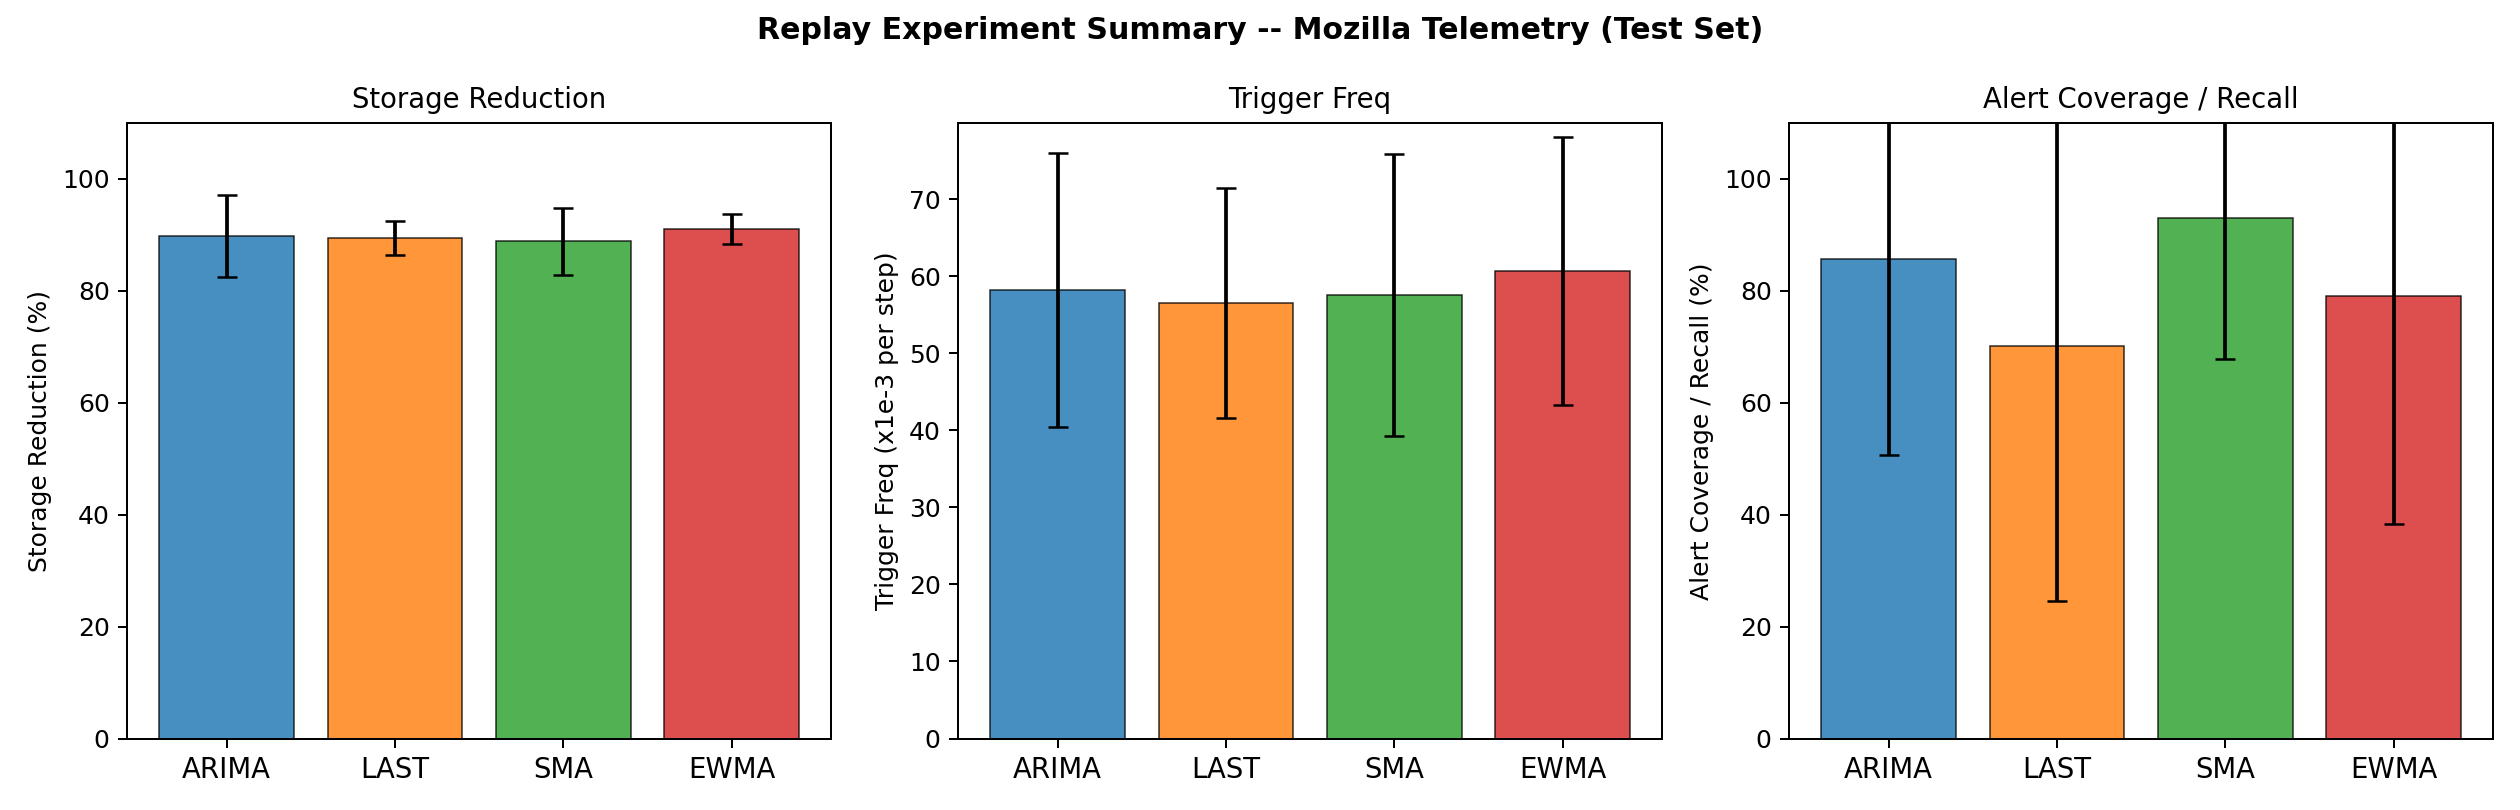
\includegraphics[width=\linewidth]{images/replay/replay_summary_panel.png}
  \caption{Boxplot distributions of storage reduction, trigger frequency, and
    alert coverage across 214 signatures for the four statistical detectors.}
  \label{fig:replay_panel}
\end{figure}

\subsection{Efficiency Frontier Analysis}\label{sec:replay:frontier}

Figure~\ref{fig:efficiency_frontier} plots storage reduction against alert
coverage for each of the four statistical detectors, revealing the
storage--coverage Pareto frontier.

\begin{figure}[H]
  \centering
  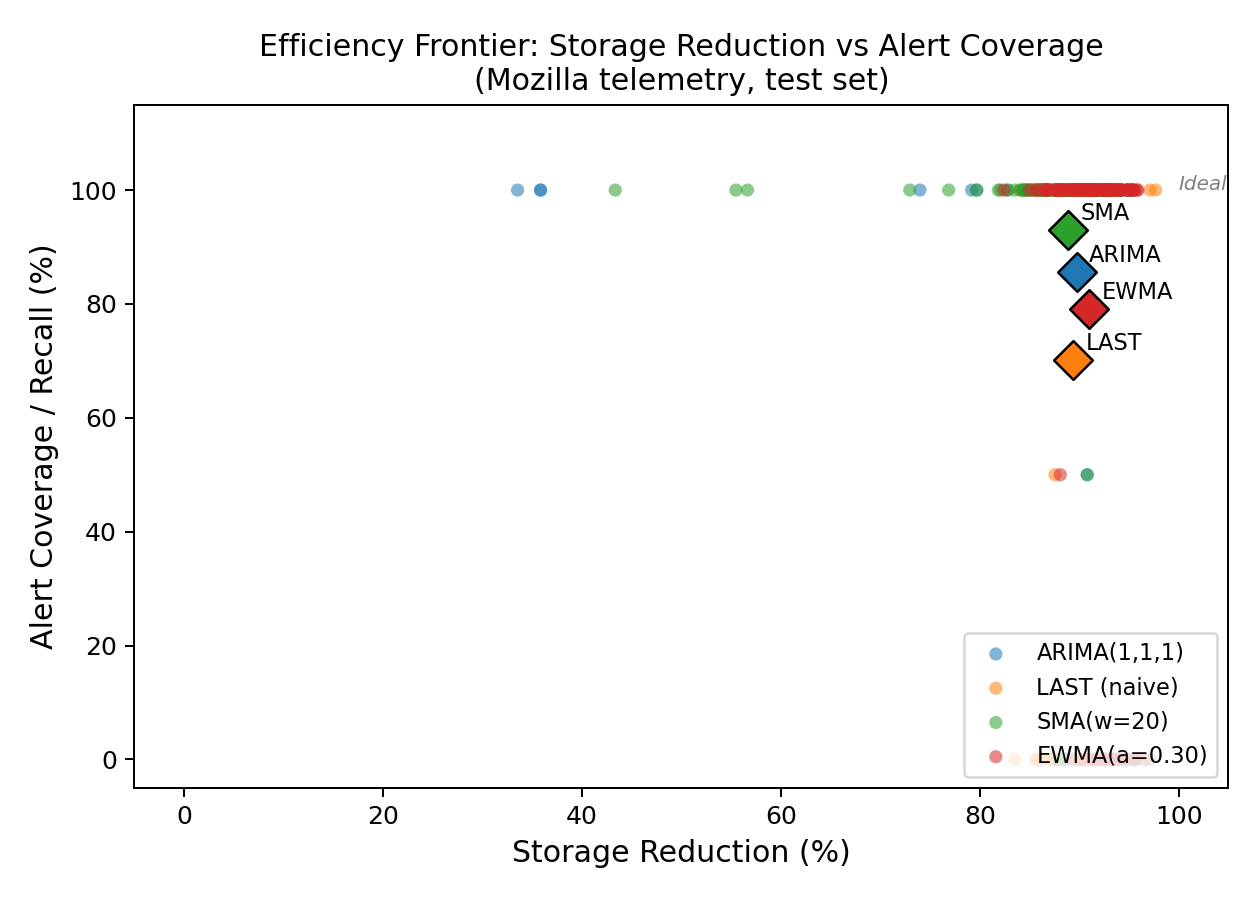
\includegraphics[width=\linewidth]{images/replay/replay_efficiency_frontier.png}
  \caption{Efficiency frontier: storage reduction vs.\ alert coverage.
    A Pareto-optimal detector lies at the top-right corner.
    SMA achieves the best combined storage--coverage trade-off;
    EWMA maximises storage reduction at the cost of lower alert coverage.}
  \label{fig:efficiency_frontier}
\end{figure}

SMA dominates for coverage; EWMA dominates for storage reduction.
ARIMA represents a balanced choice: second-highest coverage (85.7\%) with
storage reduction comparable to SMA (89.75\% vs.\ 88.83\%).
LAST is dominated---it achieves neither the highest storage reduction nor
the highest coverage.

The CDF of per-signature storage reduction is shown in
Figure~\ref{fig:cdf_storage}: all four statistical methods show tight distributions
of storage reduction (85--95\%).

\begin{figure}[H]
  \centering
  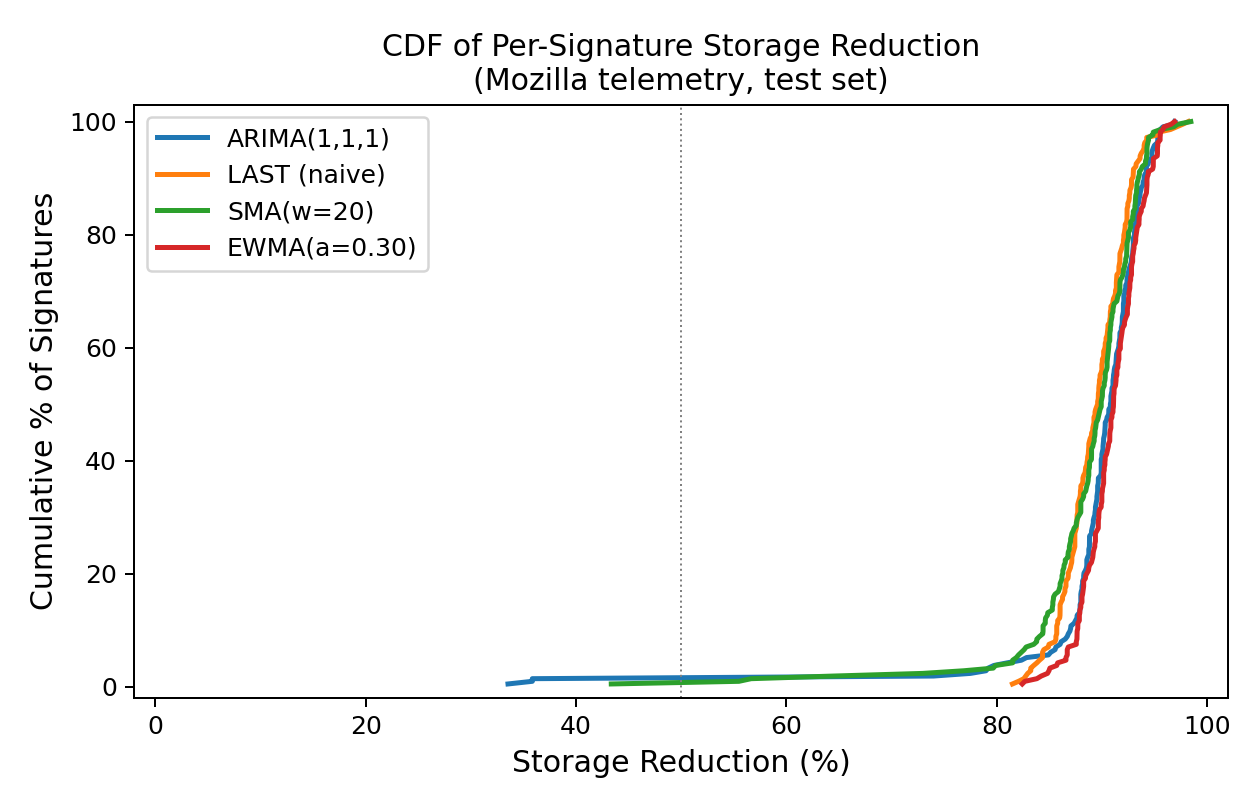
\includegraphics[width=0.9\linewidth]{images/replay/replay_cdf_storage.png}
  \caption{Cumulative distribution of per-signature storage reduction.
    All methods concentrate at 85--95\%.}
  \label{fig:cdf_storage}
\end{figure}

\textbf{RQ4 summary}: All four statistical detectors achieve a storage reduction of
$\approx 89$--91\%.
The critical differentiator is \emph{alert coverage}: SMA achieves the highest
mean per-signature alert recall (93.0\%)---it covers on average 93.0\% of a
signature's test-set alerts---while LAST achieves only 70.2\%.
SMA dominates the coverage dimension (93.0\% mean alert recall at 88.83\% storage
reduction) and is the recommended choice for deployments where alert coverage
is the primary objective.
ARIMA provides the second-highest coverage (85.7\%) at comparable storage
reduction (89.75\%), and may be preferred when an interpretable forecasting
model is required; but it should not be selected over SMA on the basis of
performance data from this benchmark.
LAST is Pareto-dominated, achieving neither the highest storage reduction
nor the highest coverage.

% ===================================================================
\section{Discussion}\label{sec:discussion}
% ===================================================================

\subsection{Operational Engine Selection}

The experimental results support the following guidance for practitioners
deploying the DAET framework.
Each recommendation below cites numbers from their source protocol explicitly:
the canonical 60\%/20\%/20\% protocol (Section~\ref{sec:three_way}) supplies
the primary F1 and storage-reduction comparisons; the calibration baseline
(Section~\ref{sec:largescale:RQ1}) supplies recall, detection-rate, and
statistical-significance results; and the replay experiment
(Section~\ref{sec:replay}) supplies alert-coverage estimates, all on the
calibration-baseline split.
Cross-protocol conclusions are stated separately in
Section~\ref{sec:discussion:scientific}.
Three deployment profiles emerge depending on accuracy objectives
and resource constraints.

\textbf{Recommended default (most deployments)}: use SMA.
\textit{Canonical 60\%/20\%/20\% protocol}: SMA achieves F1~=~0.104 on
Firefox-Android ($w=40$) and F1~=~0.085 on mozilla-beta ($w=20$)---the
leading or co-leading F1 on both datasets
(Tables~\ref{tab:three_way_fa}--\ref{tab:three_way_mb}).
\textit{Calibration baseline (70\%/30\%, 214 signatures)}: SMA ($w=20$)
achieves detection rate~96\%, mean recall~0.657, and F1~=~0.186
(Table~\ref{tab:main_results}).
\textit{Replay experiment (calibration-baseline split)}: mean per-signature
alert coverage~93.0\% and storage reduction~88.83\%
(Table~\ref{tab:replay_aggregate}).
It requires no model fitting, is deterministic, runs in 30 seconds on
all 214 signatures, and uses 16$\times$ less peak memory than ARIMA.
The optimal window ($w$) is dataset-dependent: $w=40$ gave the best
validation-set F1 on Firefox-Android under the canonical protocol, $w=20$
on mozilla-beta canonical and on the calibration baseline; deployments
should validate $w$ on a held-out segment.

\textbf{If explicit trend modelling or extensibility is required}: use
ARIMA(1,1,1).
Under the calibration baseline (70\%/30\%), ARIMA is not significantly
different from SMA in F1 ($p=0.547$) or precision ($p=0.652$); under
the canonical 60\%/20\%/20\% protocol, ARIMA falls behind SMA in F1
($p=0.004$, Firefox-Android, Table~\ref{tab:can_wil_fa}).
It significantly outperforms LAST on both protocols.
ARIMA provides a statistically motivated prediction model that distinguishes
gradual workload evolution from sudden performance regressions.
ARIMA(1,1,1) can be extended to ARIMA(p,d,q) by adaptive order selection
(AIC/BIC), allowing tuning to the autocorrelation structure of specific
signatures.
Teams should be aware of the 27$\times$ runtime cost relative to SMA
(Table~\ref{tab:compute_cost}) when making this choice.

\textbf{If storage reduction is the primary constraint}: use EWMA on
Firefox-Android.
With tuned $\alpha=0.05$ (selected via the extended grid
$\{0.01, 0.02, 0.03, 0.05, 0.10, \ldots, 0.50\}$ and confirmed as an interior
optimum; Section~\ref{sec:three_way}), EWMA achieves
higher storage reduction than SMA on Firefox-Android (89.4\% vs.\ 88.3\%),
while matching SMA in F1 (0.103 vs.\ 0.104) and maintaining comparable
detection quality.
On mozilla-beta, the margin reverses: SMA achieves 88.8\% storage reduction
vs.\ EWMA's 88.5\%, so the storage advantage is dataset-dependent and
shouldn't be taken as a universal rule.
EWMA with $\alpha=0.05$ is a practical alternative to SMA when higher
storage efficiency is a priority and the deployment context matches
Firefox-Android characteristics.

\textbf{LAST should generally be avoided}: it is significantly worse than
all other methods in precision, recall, and F1, and achieves the lowest
alert coverage (70.2\%) in the replay experiment.

\textbf{If a learned Transformer predictor is operationally preferred}:
use the compact Transformer under the 60\%/20\%/20\% protocol with
dataset-specific HP tuning (Section~\ref{sec:three_way}).
On Firefox-Android (WINDOW=20, $d_{\text{model}}=16$), five seeds yield
F1~=~0.105~($\pm$0.002) and detection rate 74.4\%---competitive with
tuned SMA.
On mozilla-beta (WINDOW=10, $d_{\text{model}}=32$), F1~=~0.079~($\pm$0.001)
and detection rate 89.8\%.
Storage reduction is lower (67--71\% vs.\ 88--90\% for classical methods)
because the learned predictor activates trace-on windows more frequently
at the standard anomaly-score threshold; practitioners should calibrate the
threshold for storage-constrained deployments.

\subsection{ARIMA vs.\ SMA: Why Not Simply Use SMA?}

A natural question arises: if SMA and ARIMA are not significantly different in
F1 and precision on the calibration baseline (Wilcoxon $p > 0.5$;
Section~\ref{sec:largescale:RQ2}), and SMA leads on recall and detection rate
(also calibration baseline), why retain ARIMA as a reference engine?

We identify three engineering-motivated reasons:
(1)~SMA's moving average generates a prediction only after the window is fully
populated and reacts symmetrically to both up and down deviations.
ARIMA(1,1,1)'s integrated first-order model can capture monotonic trends
(e.g., gradual CPU drift) and will continue predicting along the new trend
after a level shift, thereby reducing spurious alarms for organic load growth.
(2)~In settings where non-stationarity is pronounced (servers with daily
seasonality, progressive memory leaks), the integrated component of ARIMA
provides a systematic de-trending mechanism that SMA lacks.
(3)~ARIMA(1,1,1) can be extended to ARIMA(p,d,q) by adaptive order
selection (AIC/BIC), allowing the system to be tuned to the
autocorrelation structure of each specific signature.

Importantly, these reasons are conceptual and engineering-oriented, not
empirical: the current benchmark does not provide evidence that ARIMA's
trend-modelling advantage manifests in measurably better detection on
Mozilla telemetry.
Readers who prioritise measured accuracy over interpretability or
extensibility should consider SMA as the deployment default.

\subsection{When SMA Is the Better Choice}

SMA retains the highest recall (0.657), detection rate (96\%), and alert
coverage in the replay experiment (93\%) among all methods on the
calibration baseline (Section~\ref{sec:largescale:RQ1}).
Under the canonical 60\%/20\%/20\% protocol (Section~\ref{sec:three_way}),
SMA ($w=40$) achieves F1~=~0.104 on Firefox-Android, and EWMA ($\alpha=0.05$)
matches it at F1~=~0.103 with marginally higher storage reduction.
The $\alpha=0.05$ selection is confirmed as an interior optimum by an extended
grid down to $\alpha=0.01$ (Section~\ref{sec:three_way}).
Deployment teams requiring maximum recall and alert coverage should prefer
SMA, with the window validated on a held-out segment:
\begin{itemize}
  \item Highest recall (0.657) and detection rate (96\%) among all methods
    \textit{(calibration baseline, Section~\ref{sec:largescale:RQ1})}.
  \item Highest replay alert coverage (93.0\%)
    \textit{(replay experiment, calibration-baseline split,
    Table~\ref{tab:replay_aggregate})}.
  \item F1~=~0.104 (Firefox-Android, $w=40$) and 0.085 (mozilla-beta, $w=20$)
    \textit{(canonical 60\%/20\%/20\% protocol,
    Tables~\ref{tab:three_way_fa}--\ref{tab:three_way_mb})}.
  \item Zero training time (deterministic, $O(1)$ memory).
\end{itemize}
Across both protocols, SMA is consistently the highest-recall and
highest-coverage method; the optimal window differs by dataset and protocol
and should be set by validation.
For deployments where storage reduction is also a priority,
EWMA($\alpha=0.05$) achieves comparable canonical F1 to SMA
(Firefox-Android: 0.103 vs.\ 0.104; mozilla-beta: 0.083 vs.\ 0.085)
with 89.4\%--88.5\% storage reduction vs.\ SMA's 88.3\%--88.8\%;
however, EWMA's replay alert coverage (79.0\%) is lower than SMA's (93.0\%),
so the trade-off is explicit.

\subsection{Precision Ceiling and False-Positive Audit}\label{sec:discussion:fp}

Precision is low ($<0.12$) for all methods.
This is inherent to the evaluation benchmark: Treeherder regression alerts
are produced by a different detection algorithm (Bayesian change-point
detection), and many short performance excursions that DAET detects may
be \emph{real} anomalies that did not persist long enough for Mozilla's
system to raise a formal regression ticket.
The Treeherder-agreement precision therefore understates true anomaly
precision to an unknown but potentially significant degree.

To provide a concrete bound on how many ``false positives'' may be
genuine anomalies, we conducted a targeted heuristic audit of the SMA and
EWMA detectors---the two strongest classical methods---on the
calibration-baseline test set (Firefox-Android, 70\%/30\% split).
We drew a stratified random sample of 30~FP intervals per method
(seed~42), then applied the following documented labeling criteria to
each interval based solely on observable signal properties:
\begin{itemize}
  \item \emph{Likely genuine anomaly}: interval spans $\geq 3$
    consecutive detection steps \emph{and} peak anomaly score
    $\geq 0.50$---persistence and signal strength jointly suggest
    a real performance shift rather than a transient spike.
  \item \emph{Likely noise}: single-step interval ($= 1$ step)
    \emph{and} peak score $< 0.50$---characteristic of measurement
    artefacts or random threshold crossings.
  \item \emph{Unclear}: all other cases (e.g., 2-step intervals,
    or sustained but moderate-score detections).
\end{itemize}

\begin{table}[tbp]
\centering
\begin{tabular}{lccc}
\toprule
Method & Likely genuine & Likely noise & Unclear \\
\midrule
SMA  (n=30) & 7~~(23\%) & 21~~(70\%) & 2~~(7\%) \\
EWMA (n=30) & 7~~(23\%) & 22~~(73\%) & 1~~(3\%) \\
\bottomrule
\end{tabular}
\caption{Heuristic audit of 30 randomly sampled false-positive detection
  intervals per method (SMA and EWMA, calibration-baseline test set,
  Firefox-Android). Labels are assigned by documented signal-property
  criteria; see Section~\ref{sec:discussion:fp}.
  ``Likely genuine'' intervals meet the persistence and score criteria
  but were not matched by Treeherder, suggesting the true anomaly
  precision is meaningfully higher than the Treeherder-agreement
  precision reported in the main tables.}
\label{tab:fp_audit}
\end{table}

As Table~\ref{tab:fp_audit} shows, approximately 23\% of sampled
FP intervals (7/30 for both SMA and EWMA) exhibit characteristics
consistent with genuine but unlabelled performance excursions.
The majority (70--73\%) are single-step, moderate-strength events
consistent with noise or transient measurement artefacts.
This result implies that \emph{true anomaly precision} for these methods
may be meaningfully higher than the Treeherder-agreement precision
reported in the main results tables.
It also provides a concrete bound on the precision interpretation:
a rough upper-bound estimate of true anomaly precision can be
approximated as: Treeherder-agreement precision $+$ estimated genuine
FP rate $\times$ $(1 - $ Treeherder-agreement precision$)$.

We distinguish two precision concepts throughout:
``Treeherder-agreement precision'' (what Tables~\ref{tab:main_results}--\ref{tab:three_way_mb} report)
and ``true anomaly precision'' (unknowable from Treeherder labels alone).
A full validation of true anomaly precision would require cross-referencing
with Bugzilla regression reports or a dedicated manual annotation study.
We treat this audit as directional evidence that the Treeherder proxy
understates detection quality, while acknowledging that automated
heuristics are not a substitute for expert adjudication.

\subsection{Scientific Conclusions vs.\ Deployment Recommendations}\label{sec:discussion:scientific}

All results in this paper are \emph{Treeherder-agreement metrics}: they
measure how well each detector's binary output coincides with Mozilla's
automated Bayesian alerting, not true anomaly precision or debugging
effectiveness.
Subject to that construct constraint, the canonical evaluation
(Section~\ref{sec:three_way}) shows that SMA and properly tuned EWMA lead
on Treeherder-agreement F1 on both datasets; ARIMA is third; LAST is weakest.
This qualitative ranking is consistent across both repositories; however,
both benchmarks share the same CI platform and alert mechanism, so
consistency should be treated as \emph{preliminary} evidence of robustness,
not proof of cross-platform generalisation.

The evidence does not show that any single method is universally best.
Results are confined to Mozilla Treeherder data from one organisation and
one operating period; generalisation to other systems, seasonality regimes,
or monitoring platforms requires further evaluation.
Deployment guidance is in the Operational Engine Selection subsection above
(Section~\ref{sec:discussion}); statistical support for the ranking is in
Section~\ref{sec:three_way:stats}.

% ===================================================================
\section{Threats to Validity}\label{sec:threats}
% ===================================================================

\textbf{Internal validity.}
The four case studies (Section~\ref{sec:casestudies}) are illustrative
demonstrations using known bug reports.
While the framework's candidate list was generated independently of the
bug report, the evaluation is retrospective and may not generalise to bugs
of a different character.
The canonical comparative evaluation (Section~\ref{sec:three_way})
uses a strict 60\%/20\%/20\% chronological split on two repositories with
an independent held-out validation set for SMA, EWMA, and Transformer
hyperparameter selection; the test set is evaluated exactly once.
Two further internal validity limitations remain.
First, the shared anomaly-score parameters ($\beta=0.30$, $\theta=0.30$)
are applied identically to all methods without per-method or per-dataset
tuning; the ablation study shows both parameters produce large swings in
precision/recall trade-offs, so the current ranking may shift under
individual-method optimisation of these shared parameters.
Second, the EWMA tuning grid was originally limited to
$\{0.05, 0.10, \ldots, 0.50\}$, raising the question of whether a smaller
$\alpha$ might outperform $\alpha=0.05$.
An extended grid covering $\{0.01, 0.02, 0.03, 0.05, 0.10, \ldots, 0.50\}$
was evaluated; smaller $\alpha$ values produced lower validation F1 on both
datasets (e.g., $\alpha=0.01$: val~F1~=~0.077 vs.~0.098 at $\alpha=0.05$
on Firefox-Android), confirming that $\alpha=0.05$ is an interior
optimum and the reported test-set results are globally optimal within this
grid.
The calibration baseline (Section~\ref{sec:largescale:RQ1}) replicates the
conference paper's 70\%/30\% setup but without an independent validation
hold-out, making its SMA/EWMA parameter choices an acknowledged internal
validity limitation; it is retained solely for prior-work comparison.
The bootstrap confidence intervals and Wilcoxon tests
(Section~\ref{sec:largescale:RQ2}) are computed on the calibration-baseline
per-signature scores for prior-work comparison.
Bootstrap confidence intervals and Wilcoxon signed-rank tests on the
canonical 60\%/20\%/20\% test data are reported in
Section~\ref{sec:three_way:stats}
(Tables~\ref{tab:can_ci_fa}--\ref{tab:can_wil_mb}).
The compact Transformer hyperparameters were tuned on the held-out
validation set; the test set was evaluated once.
Results are reported in Section~\ref{sec:three_way} and
Tables~\ref{tab:three_way_fa}--\ref{tab:three_way_mb}:
on Firefox-Android the compact Transformer achieves F1~=~0.105~($\pm$0.002)
and detection rate 74.4\%; on mozilla-beta F1~=~0.079~($\pm$0.001), slightly
below tuned SMA and EWMA.

\textbf{Construct validity.}
The central construct limitation---that all metrics measure
\emph{Treeherder-alert agreement} rather than true anomaly precision or
debugging effectiveness---is discussed in depth in the Precision Ceiling
and Scientific Conclusions subsections of Section~\ref{sec:discussion}.
In brief: Treeherder's Bayesian alerts are an imperfect ground truth
(they may miss transient regressions or include noise from infrastructure
changes), and the paper does not show that DAET improves engineer
productivity or reduces time-to-root-cause.
Because all four statistical detectors use the same evaluation protocol,
the \emph{comparative} rankings are unaffected by this construct choice;
absolute precision values should be read as ``Treeherder-agreement
precision'' only.
A heuristic audit of 30 sampled FP intervals per method (SMA and EWMA)
found that $\approx$23\% exhibit characteristics of genuine but unlabelled
performance excursions; the majority (70--73\%) are single-step
moderate-strength events consistent with noise
(Section~\ref{sec:discussion:fp}, Table~\ref{tab:fp_audit}).
This suggests that Treeherder-agreement precision understates true anomaly
precision, though automated heuristics are not a substitute for expert adjudication.
The $\tau=5$-sample tolerance window introduces matching leniency, but
since it is applied uniformly across all methods, comparative conclusions
are unaffected.

\textbf{External validity.}
The evaluation uses two Mozilla Treeherder repositories (Firefox-Android and
mozilla-beta); both are from the same organisation and CI platform, which
limits generalisability to other applications, tracing granularities,
or monitoring infrastructures.
Furthermore, because all metrics measure agreement with Treeherder alerts
rather than ground-truth anomaly validity, the consistent qualitative ranking
across both repositories should be treated as \emph{preliminary}, not
conclusive, evidence of cross-dataset robustness: it is possible that
both benchmarks share the same systematic bias relative to true anomaly
ground truth.
Validation on external CI systems using an independent ground truth
(e.g., manually adjudicated or Bugzilla-confirmed regressions) is
required before stronger generalisability claims can be made.
The replay experiment simulates storage savings analytically; actual
deployment savings depend on storage backend, compression, and I/O scheduling.

\textbf{Conclusion validity.}
Statistical tests are reported for both the calibration baseline
(Section~\ref{sec:largescale:RQ2}, Wilcoxon on 214 paired observations)
and the canonical 60\%/20\%/20\% test set
(Section~\ref{sec:three_way:stats}, Wilcoxon on 342 Firefox-Android
and 1{,}477 mozilla-beta observations).
The Bonferroni-corrected threshold for six pairwise comparisons is
$\alpha/6 = 0.0083$.
All conclusions stated as significant in
Tables~\ref{tab:can_wil_fa}--\ref{tab:can_wil_mb}
meet this stricter bound.
The larger $n$ for the canonical tests ($342$ and $1{,}477$)
provides substantially more power than the calibration-baseline $n=214$;
the key qualitative finding that SMA~$\approx$~EWMA and both outperform
LAST is confirmed at $p < 0.001$ on both datasets.

% ===================================================================
\section{Conclusion}\label{sec:conclusion}
% ===================================================================

This paper extended the Dynamic Adaptive Execution Tracing (DAET) framework
originally introduced in~\cite{10197790} with five new contributions:
a large-scale comparative evaluation of four classical change-detection engines,
a compact Transformer encoder under fair multi-seed protocol, a formal
statistical analysis, a trace-on replay experiment, and a
three-way chronological split experiment.
The journal contribution is positioned as an \emph{empirical comparative
extension}: the core DAET framework architecture was established in the
conference paper; this work provides the large-scale prospective validation
and comparative detector study that was explicitly deferred as future work.

The framework's three-phase architecture---function selection via
family-group analysis and CoV ranking; change detection via a pluggable
change-detection engine with a dynamic anomaly-score threshold; and
trace-configuration gating---was
validated qualitatively through four Firefox Bugzilla case studies and
quantitatively via a unified 60\%/20\%/20\% pipeline on 342 Firefox-Android
and 1{,}477 mozilla-beta Treeherder telemetry signatures across five method
families; a calibration baseline on 214 signatures under the conference paper's
70\%/30\% setup is also reported for prior-work comparison.

The canonical evaluation (Section~\ref{sec:three_way}) establishes the
primary result: under a fair 60\%/20\%/20\% chronological protocol with
independent validation tuning, SMA and EWMA lead on Treeherder-agreement
F1 on both datasets; ARIMA is third; LAST is weakest.
The qualitative ranking (SMA~$\approx$~EWMA~$\geq$~ARIMA~$>$~LAST) is
consistent across both Mozilla repositories, providing \emph{preliminary}
evidence of robustness within the Mozilla CI context; stronger
generalisation claims require validation against an independent ground truth.
The compact Transformer (five seeds, canonical protocol, per-dataset HP tuning)
achieves competitive F1 with top classical methods on Firefox-Android and
slightly below on mozilla-beta, with low seed-to-seed variance.
An extended EWMA tuning grid ($\alpha \in \{0.01,\ldots,0.50\}$) confirmed
that $\alpha=0.05$ is an interior optimum on both datasets and the
test-set results are unchanged.
A heuristic false-positive audit of 30 sampled FP intervals per method
(SMA and EWMA) found that $\approx$23\% exhibit characteristics of genuine
but unlabelled performance excursions, providing directional evidence that
Treeherder-agreement precision understates true anomaly detection quality
(Section~\ref{sec:discussion:fp}).
Supporting evidence---calibration-baseline recall and Wilcoxon tests,
supplementary replay storage and coverage estimates on the calibration-baseline
split, and ablation parameter sensitivity---is reported in
Sections~\ref{sec:largescale}--\ref{sec:replay}; deployment guidance is
in Section~\ref{sec:discussion}.
All conclusions are Treeherder-agreement results; actual debugging
effectiveness requires further validation (Section~\ref{sec:threats}).

\textbf{Future work.}
Open directions include:
(i)~re-implementing the replay experiment within the unified pipeline
(\texttt{run\_full\_evaluation.py}) to fully consolidate the deployment
evidence under the canonical 60\%/20\%/20\% protocol;
(ii)~extending the heuristic FP audit (Section~\ref{sec:discussion:fp})
to a fully expert-adjudicated sample cross-referenced with Bugzilla
regression reports to obtain a calibrated estimate of true anomaly precision;
(iii)~extending the framework to seasonally non-stationary workloads using
SARIMA or STL decomposition;
(iv)~integrating anomaly score signals directly into an observability platform
(e.g., Prometheus/Grafana) for real-time deployment;
(v)~evaluating the framework on additional CI/CD pipelines beyond Mozilla
Firefox; and
(vi)~extending the dual-dataset evaluation to additional Mozilla CI projects
and to external production systems beyond Firefox to assess cross-domain
generalisability of the qualitative ranking.

% ===================================================================
\appendix
% ===================================================================

\section{Reproducibility Details for Qualitative Case Studies}\label{app:reproducibility}

This appendix records the workload and measurement specifics for the four
qualitative case studies (Section~\ref{sec:casestudies}) to support
independent replication.

\subsection*{Case Study 1 --- Apache/nmon Setup}
\begin{itemize}
  \item \textbf{Workload:} PHP script served by Apache; 30\% probability of
    loading a 50\,MB plain-text file and echoing it back, plus random
    prime-number generation for CPU load.
    Concurrent request count was stepped up fivefold (starting at 2,
    incremented by 2) over the course of the run.
  \item \textbf{Data collection command:} \verb|nmon -f -s 1 -c 3600|
    (1-second sampling interval, 3{,}600 samples = 1 hour; output written
    to the current directory rather than the terminal via the \texttt{-f} flag).
  \item \textbf{Duration:} 1 hour.
  \item \textbf{ARIMA parameters:} $\text{threshold}_{\text{ARIMA}} = 3\%$
    (both upward and downward); $\beta = 0.30$;
    $\text{threshold}_{\text{anomaly}} = 0.30$.
\end{itemize}

\subsection*{Case Studies 2 and 3 --- Firefox Application Profiling Setup}
\begin{itemize}
  \item \textbf{Firefox build:} built from source with the \texttt{perf}
    profiling flag enabled (following Mozilla's official documentation~\cite{firefoxdocumentation})
    to allow JIT-compiled code to be captured in call stacks.
  \item \textbf{Profiling tool:} Linux \texttt{perf} with 10\,ms time-slice
    snapshots to attribute execution time to individual function calls.
  \item \textbf{Profiling duration:} 20 minutes (Case Study 2 --- large/small
    PDF combinations); 15 minutes (Case Study 3 --- 3D CSS animation sequences).
  \item \textbf{Cutoff:} 5\% of all unique family-groups retained for monitoring
    (sorted by call frequency then CoV ranking).
\end{itemize}

\subsection*{Case Study 4 --- Firefox DNS/Network Profiling Setup}
\begin{itemize}
  \item \textbf{Workload:} Firefox launched repeatedly while the system DNS
    was rotated among Google's DNS, a random invalid DNS, and disconnected
    network to reproduce the DNS-resolution failure described in~\cite{cook-2022}.
  \item \textbf{Profiling tool:} Linux \texttt{perf} (same configuration as
    Case Studies 2 and 3).
  \item \textbf{Profiling duration:} 15 minutes.
  \item \textbf{Cutoff:} 5\% CoV-ranking cutoff; 289 monitored items from
    5,764 unique family-groups.
\end{itemize}

% ===================================================================
% (backmatter removed for CAS-SC)
% ===================================================================

\section*{Acknowledgements}
The authors thank the Mozilla Performance Team for making the Treeherder
telemetry dataset publicly available.

\section*{Declarations}
\textbf{Conflict of interest:}
The authors declare no conflict of interest.

\noindent\textbf{Data and code availability:}
All source code for the experimental pipeline, evaluation, ablation, replay
experiments, and figure generation is publicly available at
\url{https://github.com/ghazalkhb/Performance-Debugging}.
A tagged release corresponding to the exact version used for this paper is
provided.
The repository includes:
\begin{itemize}
  \item \texttt{requirements.txt} with pinned package versions
    (Python~3.12, statsmodels~0.13.5, numpy~1.24, pandas~2.0, scipy~1.11,
     torch~2.4.1+cpu);
  \item \texttt{run\_full\_evaluation.py}: unified dual-dataset evaluation
    pipeline that runs all five methods (ARIMA, LAST, SMA, EWMA, and
    compact Transformer) on both datasets under the 60\%/20\%/20\% protocol
    and reproduces all three-way tables and figures with a single command;
  \item preprocessing instructions for obtaining and filtering the Mozilla
    Treeherder dataset (signature matching, length filters, alert alignment);
  \item all random seeds are fixed to 42 in the bootstrap resampling;
    the detectors themselves are deterministic.
\end{itemize}
The Mozilla performance-telemetry datasets are publicly accessible via the
Treeherder API at \url{https://treeherder.mozilla.org/} under the projects
\texttt{firefox-android} and \texttt{mozilla-beta}.

% Bibliography
\bibliographystyle{cas-model2-names}
\bibliography{thesis}

\end{document}
